\section{Strato limite su placca piana}\label{c9}
La presente esercitazione si pone come obiettivo la caratterizzazione dello strato limite su placca piana mediante l'utilizzo dell'anemometria a filo caldo. In particolare, si vuole:
\begin{itemize}
    \item Misurare i profili di velocità per diverse ascisse $x$ con assegnata $U_\infty$;
    \item Caratterizzare la struttura dello strato limite:
    \begin{itemize}
        \item diagrammare i profili di velocità $u=u(x,y)$ e della deviazione standard delle fluttuazioni turbolente longitudinali $u_{rms}(x,y)$;
        \item valutare lo spessore geometrico $\delta(x)$, lo spessore di spostamento $\delta^*(x)$, lo spessore di quantità di moto $\theta(x)$ e il parametro di forma $H(x)$;
        \item verificare la condizione dello strato limite: laminare, transizionale o turbolento;
        \item diagrammare i profili di velocità media e fluttuante nella forma adimensionale: $u/U_\infty = f(y/\delta)$ e $u_{rms}/U_\infty = f(y/\delta)$.
    \end{itemize}
\end{itemize}

\subsection{Descrizione dell'esperimento}
A governare il campo di moto è il numero di Reynolds e in relazione al valore assunto localmente ($Re_{x}=U_\infty\cdot x/\nu$) lo strato limite può essere laminare oppure turbolento.
\begin{figure}[H]
    \centering
    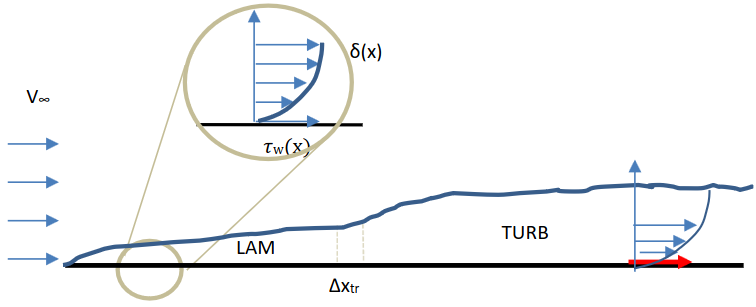
\includegraphics[width=.8\textwidth]{images/9/slimage.png}
    \caption{Rappresentazione dello strato limite}
\end{figure}

\noindent Se il numero di Reynolds locale supera il numero di Reynolds critico $Re_{cr}$ allora si ha strato limite turbolento, altrimenti si ha strato limite laminare. Dal numero di Reynolds critico si può quindi individuare la coordinata $x_{tr}$ di transizione:
\begin{equation*}
    Re_{cr}=\frac{U_\infty \cdot x_{tr}}{\nu}=5\cdot10^5
\end{equation*}
Per una placca piana posta ad incidenza nulla in un flusso senza turbolenza il numero di Reynolds critico vale $Re_{cr}\approx5\cdot10^5$. Se invece è presente turbolenza la transizione dello strato limite è anticipata, pertanto il numero di Reynolds critico risulta inferiore.\\\\
Per una data lunghezza $L$ della placca e conoscendo il valore della velocità della corrente a monte è possibile definire il numero di Reynolds globale della placca:
\begin{equation*}
    Re_L = \frac{U_\infty \cdot L}{\nu}
\end{equation*}
Nel caso di strato limite laminare la soluzione delle equazioni porta alla soluzione di Blasius, che definisce il profilo di velocità adimensionale sotto forma di tabella:
\begin{equation*}
    \eta(x,y) \approx \frac{y}{\delta(x)} = y\sqrt{\frac{U_\infty}{\nu x}} \qquad f^\prime = \frac{u}{V_\infty}
\end{equation*}
Per lo strato limite laminare sono valide le seguenti relazioni empiriche:
\begin{equation*}
    \delta(x) = \frac{5x}{\sqrt{Re_x}} \qquad \delta^*(x) = \frac{1.73x}{\sqrt{Re_x}} \qquad \theta(x) = \frac{0.664x}{\sqrt{Re_x}} \qquad H(x) = \frac{\delta^*}{\theta}
\end{equation*}
\begin{equation*}
    \tau_w(x) = 0.332 \sqrt{\frac{\rho \mu U_\infty^3}x} \qquad c_f(x) = \frac{0.664}{\sqrt{Re_x}} \qquad c_D = \frac{1.328}{\sqrt{Re_L}}
\end{equation*}
Nel caso di strato limite turbolento è presente una struttura multi-strato costituita principalmente da due regioni: inner layer ed outer layer.\\\\
L'inner layer, che copre una frazione pari al 10\%-20\% dello spessore dello strato limite $\delta$, a sua volta è costituito da tre substrati: il sottostrato viscoso, il buffer layer e la regione logaritmica.
\begin{figure}[H]
    \centering
    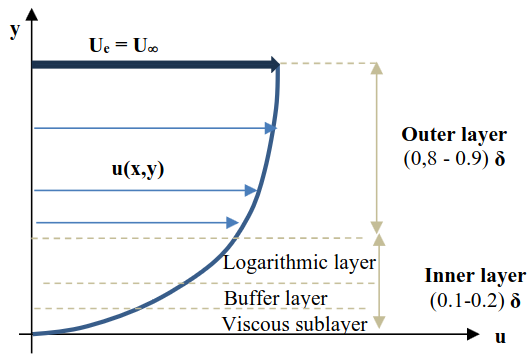
\includegraphics[width=.55\textwidth]{images/9/sltimage.png}
    \caption{Rappresentazione del profilo di velocità in uno strato limite turbolento}
\end{figure}

\noindent Per lo strato limite turbolento si definisce la velocità di attrito:
\begin{equation*}
    u_\tau = \sqrt{\frac{\tau_w}{\rho}}
\end{equation*}
E la lunghezza di attrito:
\begin{equation*}
    l_\tau = \frac{\nu}{u_\tau}
\end{equation*}
Se la velocità $u(y)$ si adimensionalizza rispetto alla velocità di attrito $u_\tau$ e la distanza da parete $y$ rispetto alla lunghezza di attrito $l_\tau$, la distribuzione di velocità si può presentare nella forma adimensionale più appropriata per lo studio dello strato limte turbolento, ovvero si esprime $u^+ = f(y^+)$. Le nuove variabili sono quindi definite come:
\begin{equation*}
    y^+ = \frac{y}{l_\tau} \qquad u^+ = \frac{u}{u_\tau}
\end{equation*}
Trattandosi di strato limite turbolento la velocità è da intendersi come velocità media nel tempo. Per il sottostrato viscoso e la regione logaritmica dell'inner layer sono definite opportune leggi di distribuzione della velocità $u^+=f(y^+)$:
\begin{itemize}
    \item Sottostrato viscoso: $0 \le y^+ \le 5$
    \begin{equation*}
        u^+ = y^+
    \end{equation*}
    \item Regione logaritmica: $30 \le y^+ \le 500$
    \begin{equation*}
        u^+ = \frac{1}{k}log(y^+) + B
    \end{equation*}
    con $k = 0.41$ (costante di Von Karman) e $B = 5.2$ (costante di Coles).
\end{itemize}

\noindent L'estremo superiore (500) della regione logaritmica in generale dipende dal numero di Reynolds e dal gradiente di pressione.
\begin{figure}[H]
    \centering
    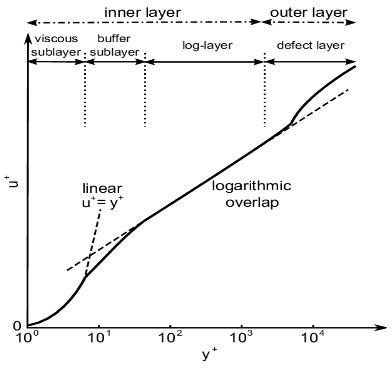
\includegraphics[width=.55\textwidth]{images/9/slinnerimage.png}
    \caption{Rappresentazione del profilo di velocità nell'inner layer}
\end{figure}

\noindent Per lo strato limite turbolento incomprimibile valgono le seguenti relazioni empiriche:\\\\
\textbf{Bassa turbolenza ($5\cdot10^5<Re<10^7$)}
\begin{equation*}
    \delta(x) = \frac{0.370x}{Re_x^{1/5}} \qquad q^*(x) = \frac{0.04625 x}{Re_x^{1/5}} \qquad \theta(x) = \frac{0.0360 x}{Re_x^{1/5}} \qquad H=\frac{\delta^*(x)}{\theta(x)}
\end{equation*}
\begin{equation*}
    \tau_w(x) = \frac{0.0288 \rho U^2}{Re_x^{1/5}} \qquad c_f = \frac{0.0576}{Re_x^{1/5}} \qquad \overline \tau_w = \frac{0.036\rho U^2}{Re_L^{1/5}} \qquad c_D = \frac{0.074}{Re_L^{1/5}}
\end{equation*}
\textbf{Alta turbolenza ($Re>10^7$)}
\begin{equation*}
    \delta(x) = \frac{0.232x}{Re_x^{1/7}} \qquad q^*(x) = \frac{0.0193 x}{Re_x^{1/5}} \qquad \theta(x) = \frac{0.0164 x}{Re_x^{1/5}} \qquad H=\frac{\delta^*(x)}{\theta(x)}
\end{equation*}
\begin{equation*}
    \tau_w(x) = \frac{0.0115 \rho U^2}{Re_x^{1/7}} \qquad c_f = \frac{0.0230}{Re_x^{1/7}} \qquad \overline \tau_w = \frac{0.0134\rho U^2}{Re_L^{1/7}} \qquad c_D = \frac{0.0295}{Re_L^{1/7}}
\end{equation*}

\subsection{Catena di misura}
La galleria del vento è del tipo a circuito aperto-aspirato con camera di prova circolare e chiusa.\\\\
All'interno della camera di prova è posta una placca piana, a contatto con le pareti della galleria in modo da rendere il flusso il più bidimensionale possibile.\\\\
La sonda a filo caldo è posizionata verticalmente in prossimità della placca piana mediante un movimentatore elettromeccanico passo-passo, in grado di spostare verticalmente la sonda di un millimetro per ogni 200 passi.\\\\
Il sistema sonda-movimentatore passo-passo, è posizionato lungo la mezzeria della galleria placca piana, ad una distanza $x$ misurata approssimativamente dal bordo di attacco.\\\\
Nella catena di misura è inoltre presente un tubo di Pitot necessario per regolare la velocità del flusso nella galleria del vento ed un sistema di acquisizione dati.
\begin{figure}[H]
    \centering
    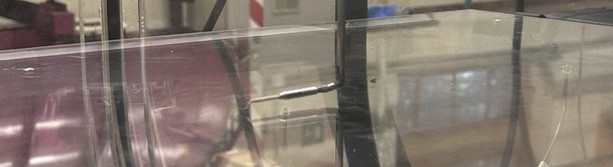
\includegraphics[width=.8\textwidth]{images/9/sonda.jpg}
    \caption{Sonda a filo caldo posizionata sulla placca piana}
\end{figure}

\begin{figure}[H]
    \centering
    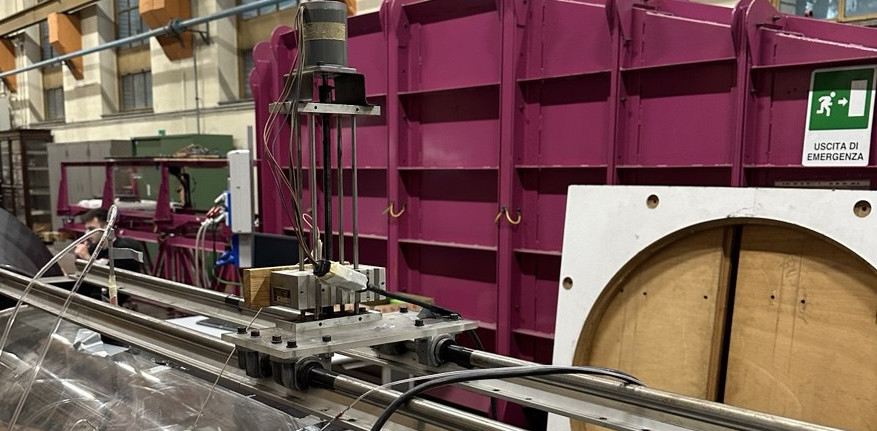
\includegraphics[width=\textwidth]{images/9/passopasso.jpg}
    \caption{Motore passo-passo e slitta per il posizionamento della sonda}
\end{figure}
\begin{figure}[H]
    \centering
    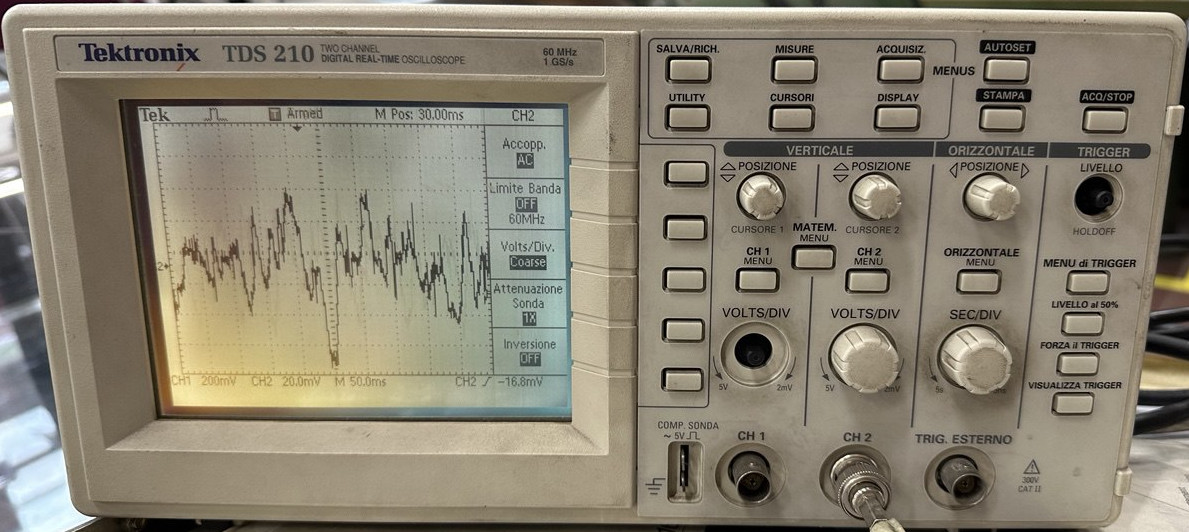
\includegraphics[width=\textwidth]{images/9/anem1.jpg}
    \caption{Anemometro}
\end{figure}

\newpage
\subsection{Procedura sperimentale}
Come prima operazione si calcola la densità e la viscosità dinamica, a partire dalla pressione e dalla temperatura ambiente, utilizzando la legge dei gas perfetti e la legge di Sutherland:
\begin{equation*}
    \rho = \frac{p_{amb}}{RT_{amb}} \qquad \mu = 1.46\cdot10^{-6} \frac{T_{amb}^{3/2}}{T_{amb}+110}
\end{equation*}
Ogni esperimento viene effettuato ad una determinata distanza $x$, misurata in modo approssimativo dal bordo d'attacco della placca piana. La galleria del vento è inoltre impostata ad una velocità costante $U_\infty$, misurata dal tubo di Pitot. Si eseguono misure su due configurazioni $(x,U_\infty)$ per ognuna delle quattro squadre, per un totale di otto configurazioni:\\
Squadra 1: ($x = 0.55$ m, $U_\infty= 8.7$ m/s), ($x = 0.9$ m, $U_\infty= 8.7$ m/s)\\
Squadra 2: ($x = 0.50$ m, $U_\infty= 10.9$ m/s), ($x = 0.9$ m, $U_\infty= 10.9$ m/s)\\
Squadra 3: ($x = 0.9$ m, $U_\infty= 11$ m/s), ($x = 0.9$ m, $U_\infty= 3.6$ m/s)\\
Squadra 4: ($x = 0.7$ m, $U_\infty= 3.1$ m/s), ($x = 0.7$ m, $U_\infty= 10.8$ m/s)\\\\
Prima di azionare la galleria del vento, è bene misurare la tensione di offset $E_0$ della sonda a filo caldo, in modo da poter ricavare la costante $A$ della legge di King per ognuna delle configurazioni:
\begin{equation*}
    E^2 = A + BU^n \qquad A = E_0^2
\end{equation*}
Come costanti $B$ ed $n$ si utilizzano quelle ricavate durante l'attivita precedente.\\\\
La prima posizione della sonda è ad approssimativamente mezzo millimetro di distanza $y$ dalla placca piana. In questa posizione si acquisiscono i dati di tensione in uscita dall'anemometro ad una determinata frequenza di campionamento $f_s=200$ Hz per un periodo $T=30$ s.\\\\
La sonda non può avvicinarsi troppo alla placca, perché in caso di contatto, questa potrebbe rompersi. Inoltre, poiché il supporto che tiene la sonda non è infinitamente rigido, il flusso d'aria della galleria ne induce delle vibrazioni, che fanno oscillare la sonda a filo caldo. Se la sonda è troppo vicina alla placca, le oscillazioni possono indurre un contatto e quindi portare al danneggiamento della sonda.\\\\
Una volta acquisiti i primi dati, mediante il sistema di azionamento del motore passo-passo, si aumenta con precisione la distanza della sonda a filo caldo dalla placca piana $y$ e si acquisiscono nuovamente i dati.\\\\
Per ogni configurazione si ottengono quindi $N = f_s\cdot T$ dati campionati ad ogni distanza $y$ considerata.\\\\
Infine, per eseguire un'analisi in frequenza, si esegue una misura ad un'elevata frequenza di campionamento ($f_s=30$ kHz, per la quarta squadra $f_s=20$ kHz) per un periodo di un minuto (55 secondi per la squadra 4).

\subsection{Analisi dati}
L'analisi dati per la presente attività è condotta con l'ausilio di un codice Python, riportato in appendice \ref{b9}.\\\\
Ad ogni valore di tensione in uscita dall'anemometro rilevato, si associa un valore di velocità mediante l'utilizzo della legge di King:
\begin{equation*}
    U_i = \left( \frac{E_i^2-A}B \right)^{1/n}
\end{equation*}
Per ogni stazione di acquisizione, si calcola il valore medio $u(y)$ e la deviazione standard $u_{rms}(y)$ della velocità:
\begin{equation*}
    u(y) = \frac{1}{N}\sum_{i=1}^{N} U_i \qquad u_{rms}(y) = \sqrt{\frac{1}{N}\sum_{i=1}^{N}{\left(U_i - u(y)\right)^2}}
\end{equation*}
A questo punto è già possibile tracciare dei diagrammi dimensionali dei profili di velocità e di deviazione standard:
\begin{figure}[H]
    \centering
    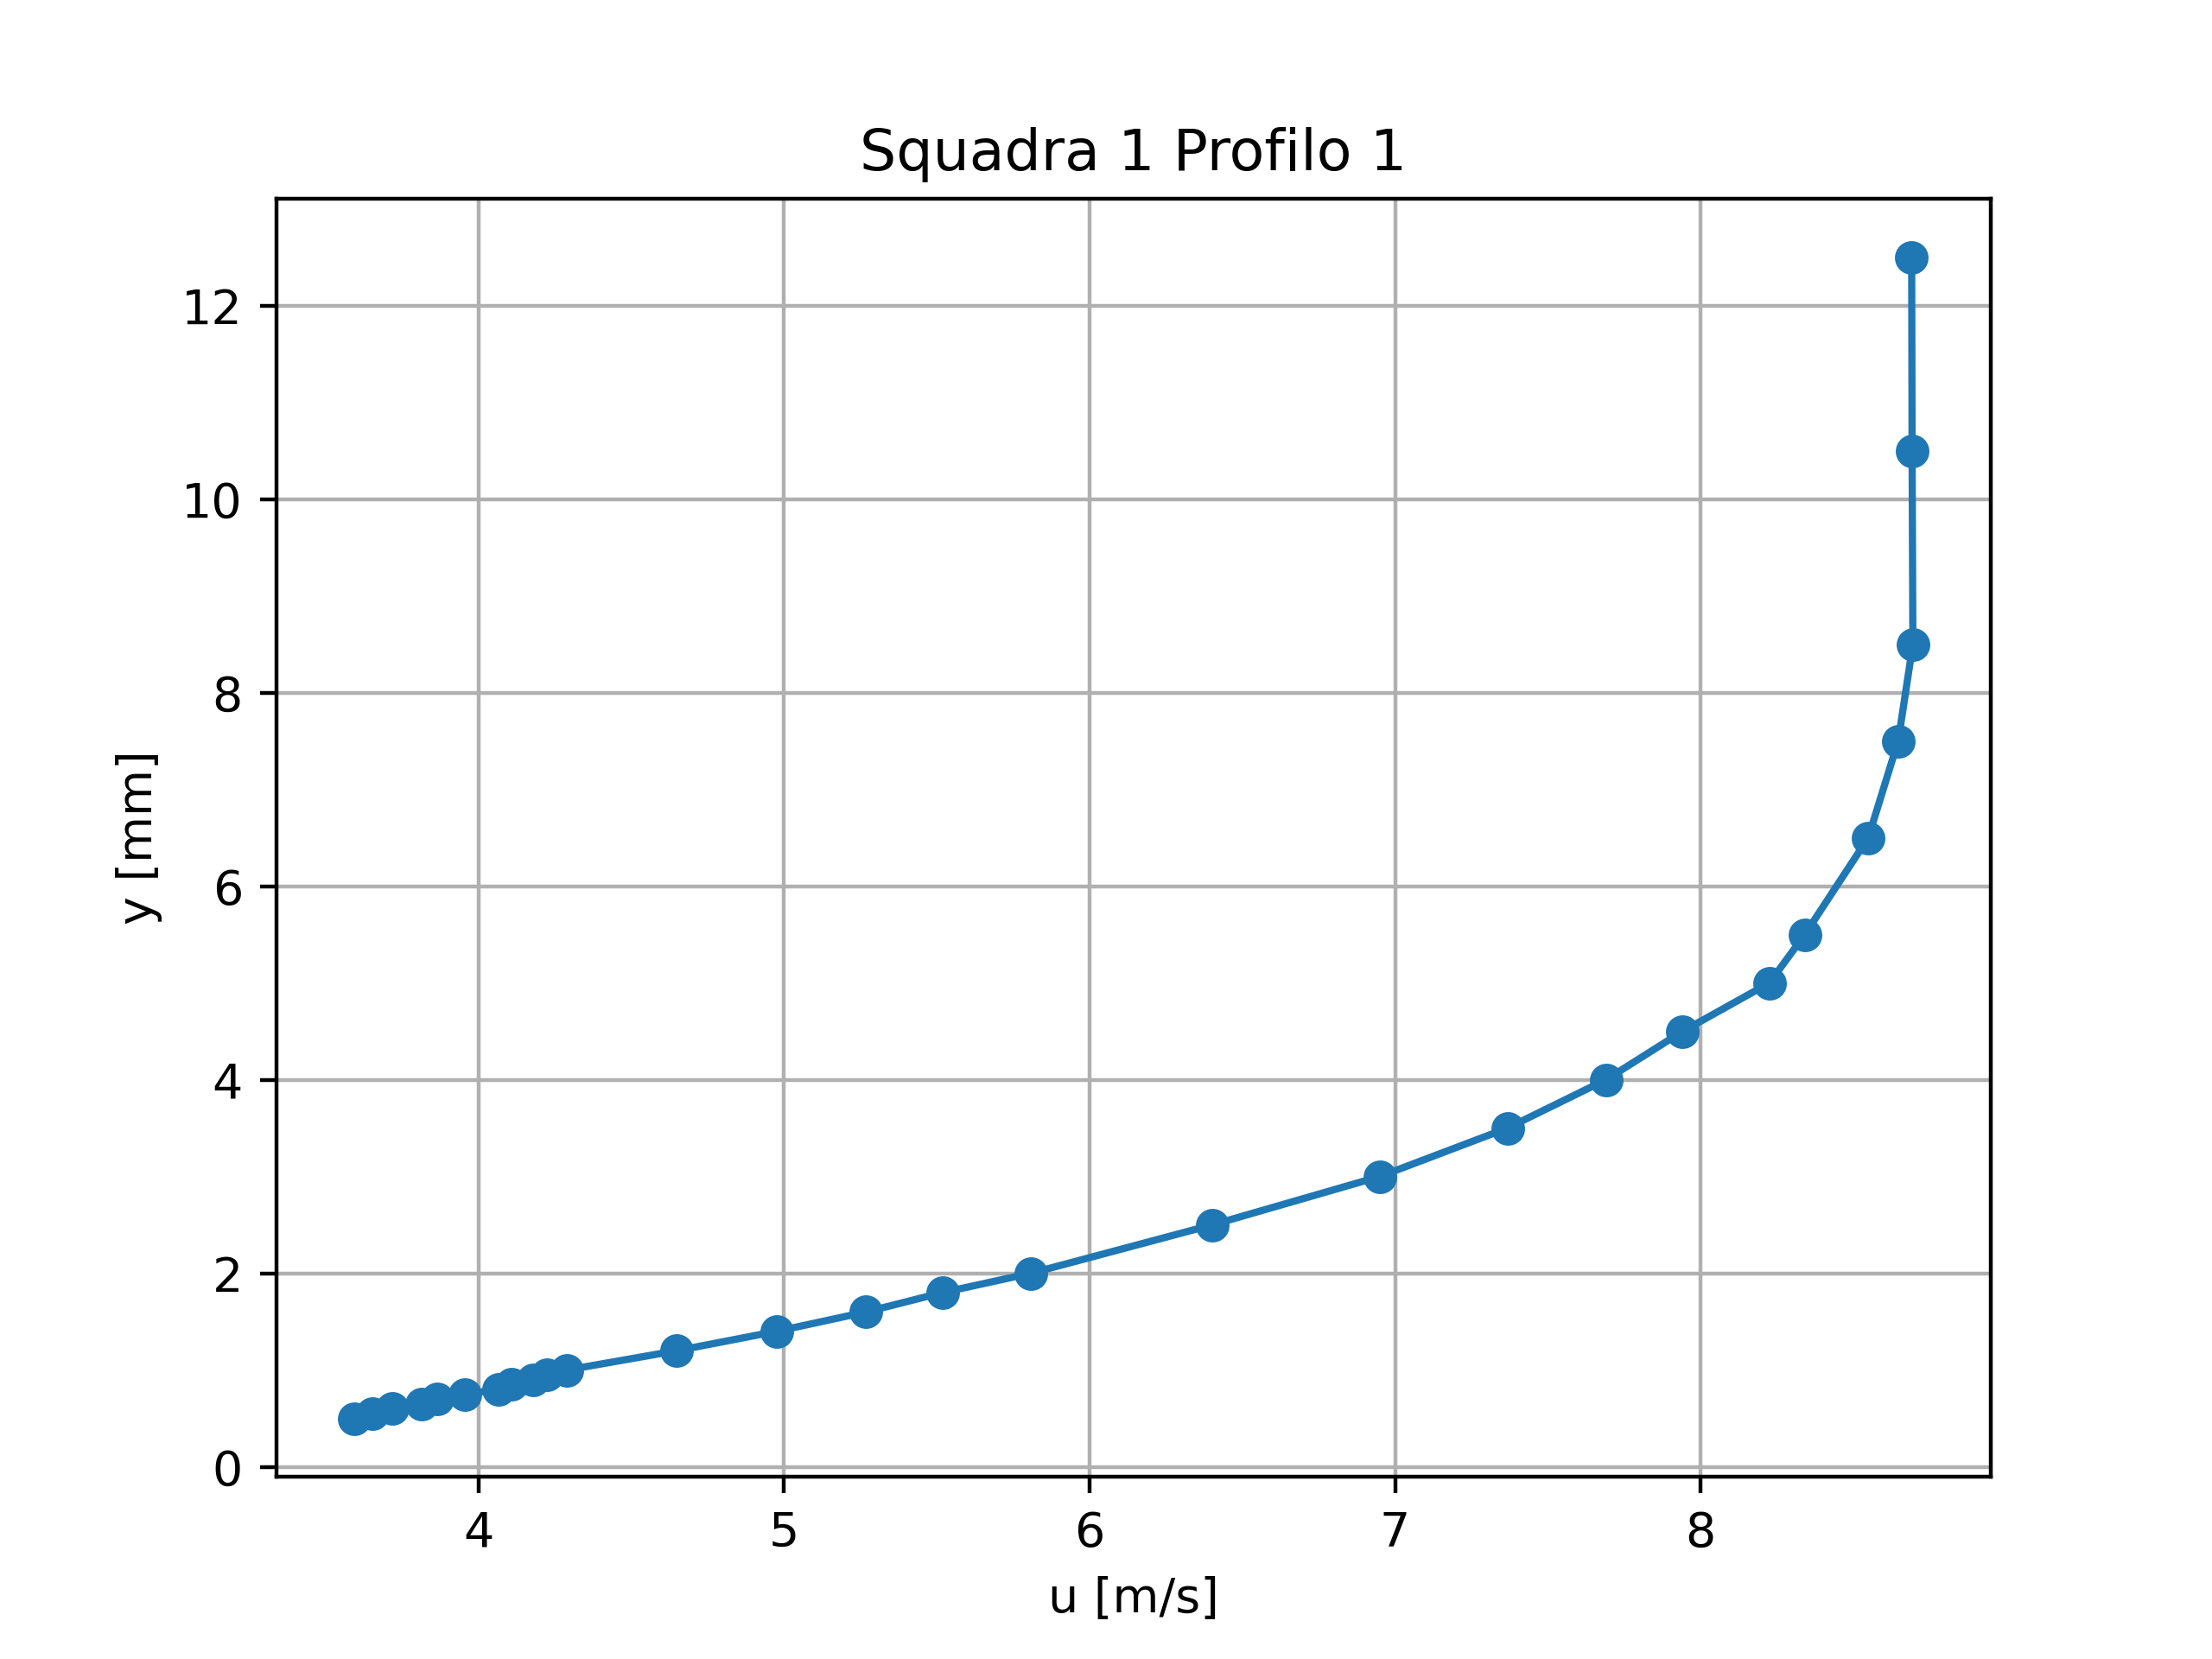
\includegraphics[width=.49\textwidth]{images/9/sq1p1.png}
    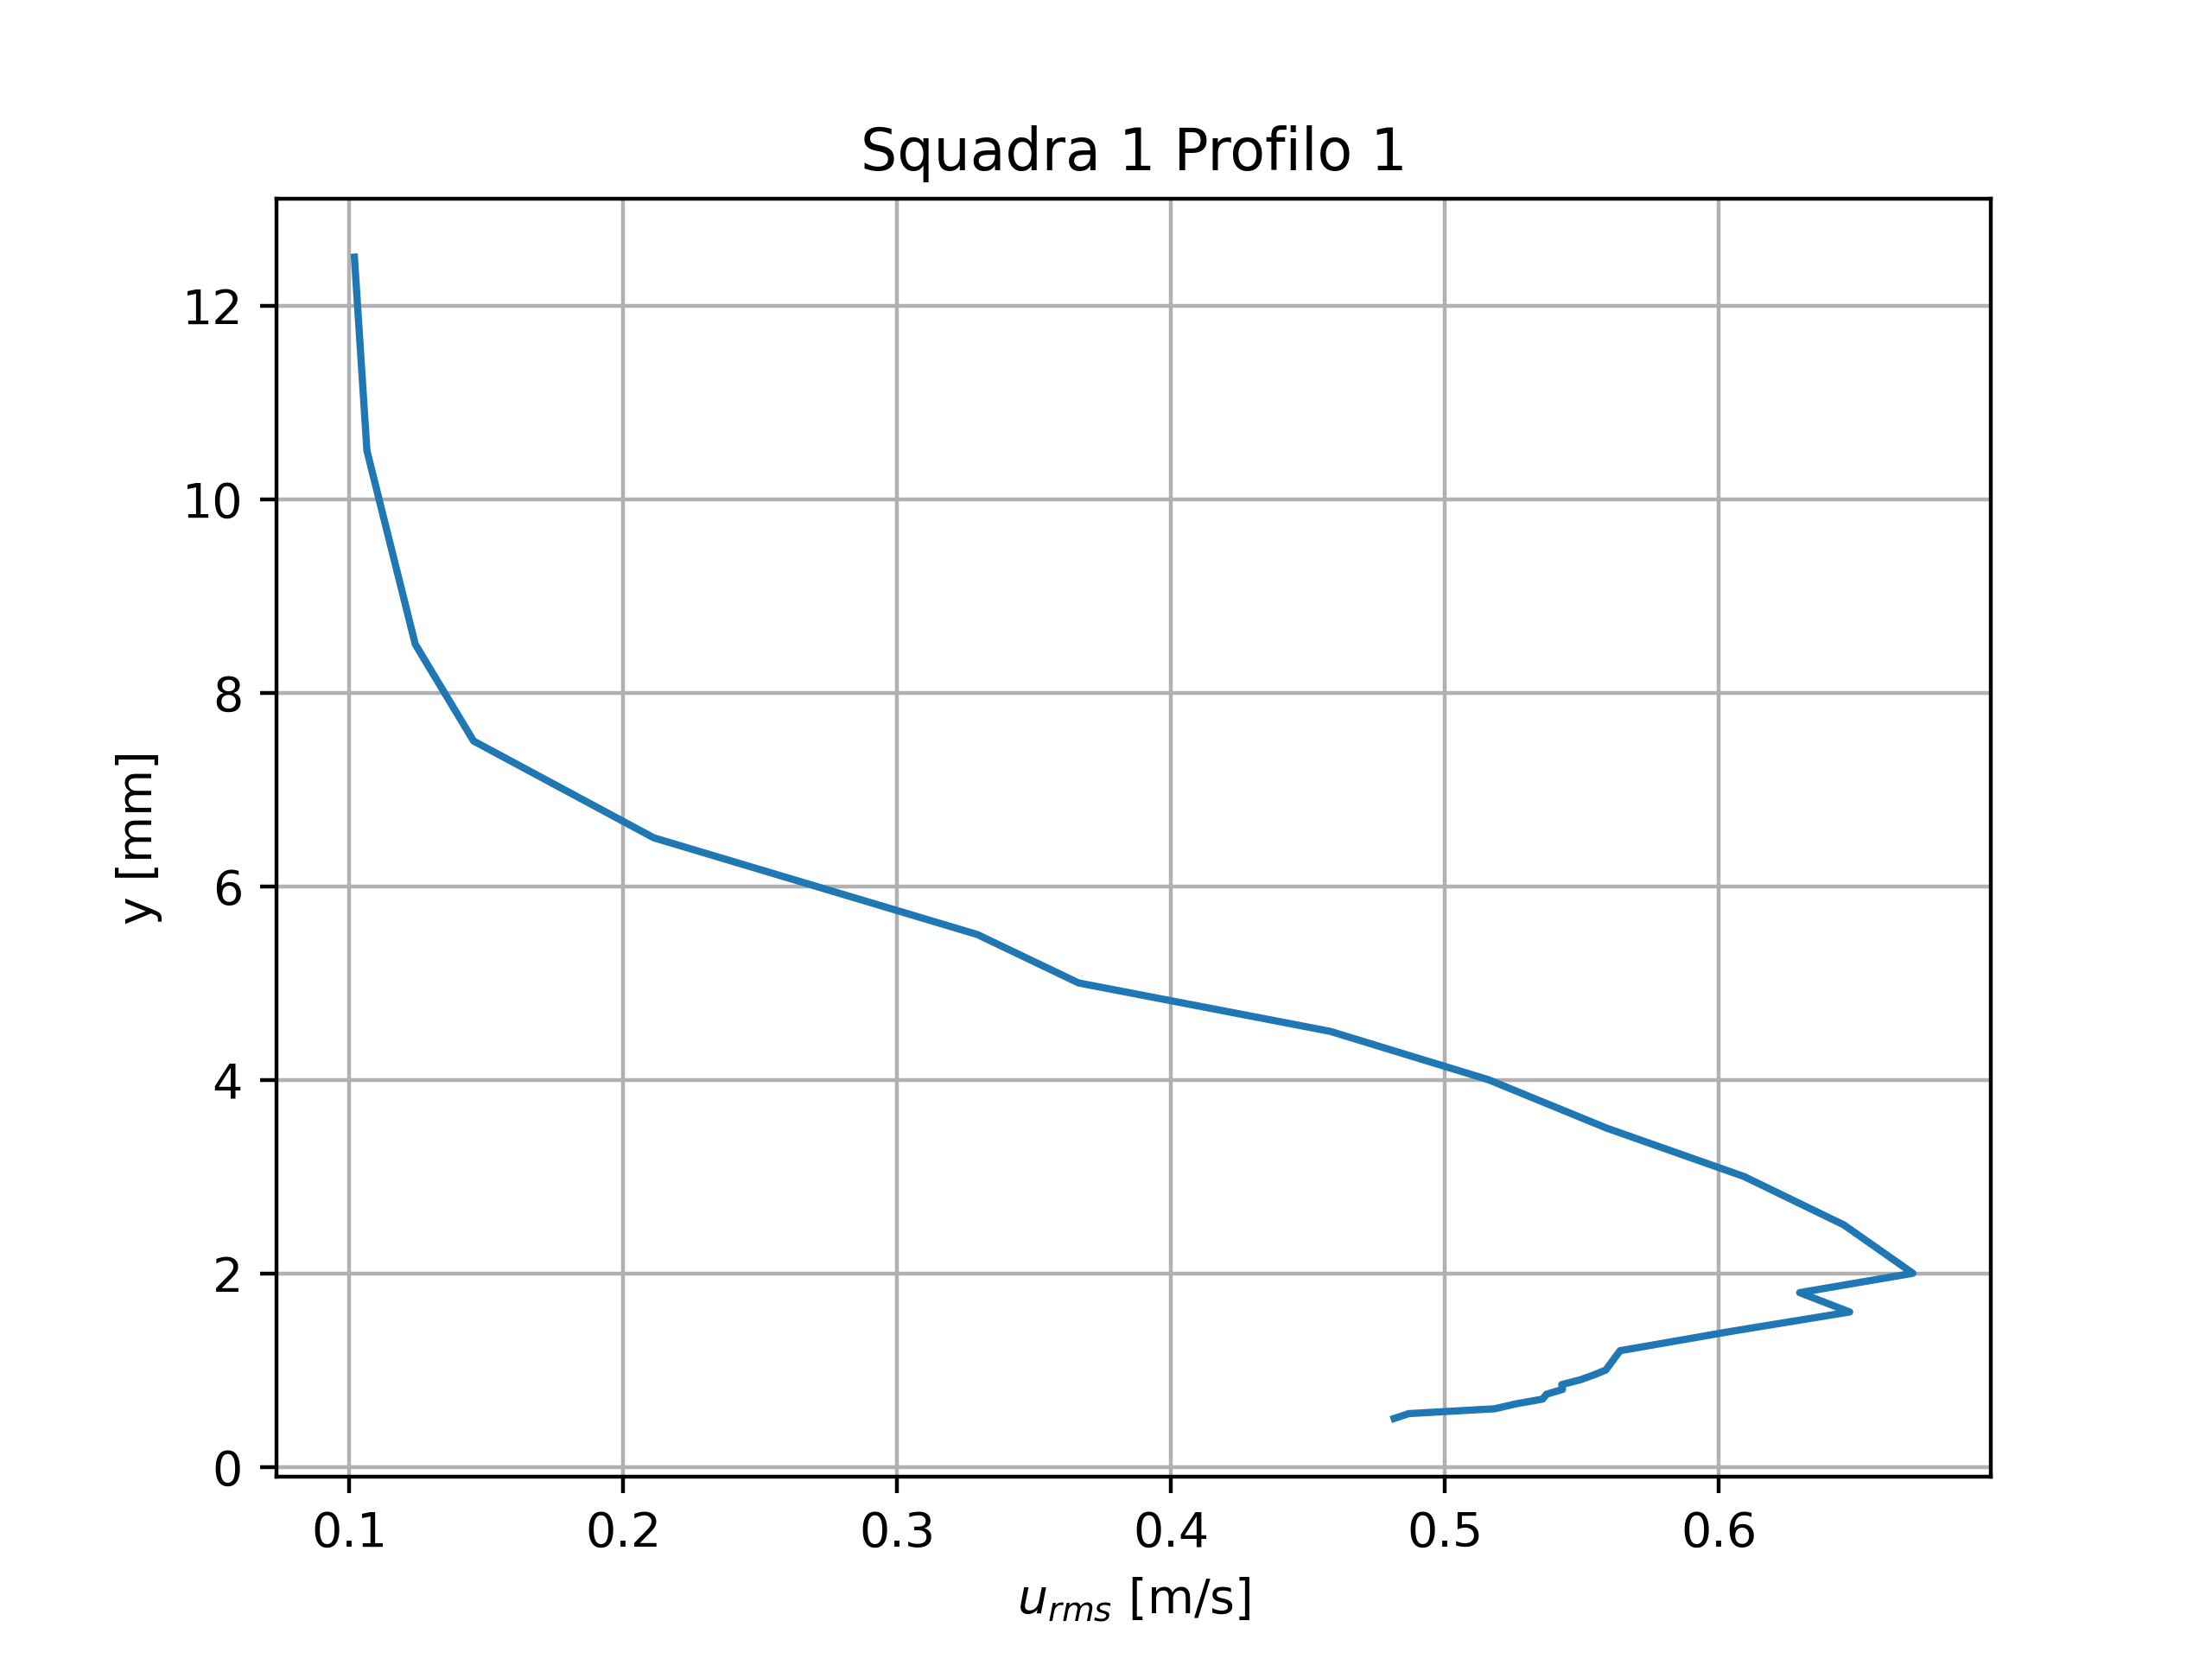
\includegraphics[width=.49\textwidth]{images/9/sq1p1rms.png}
    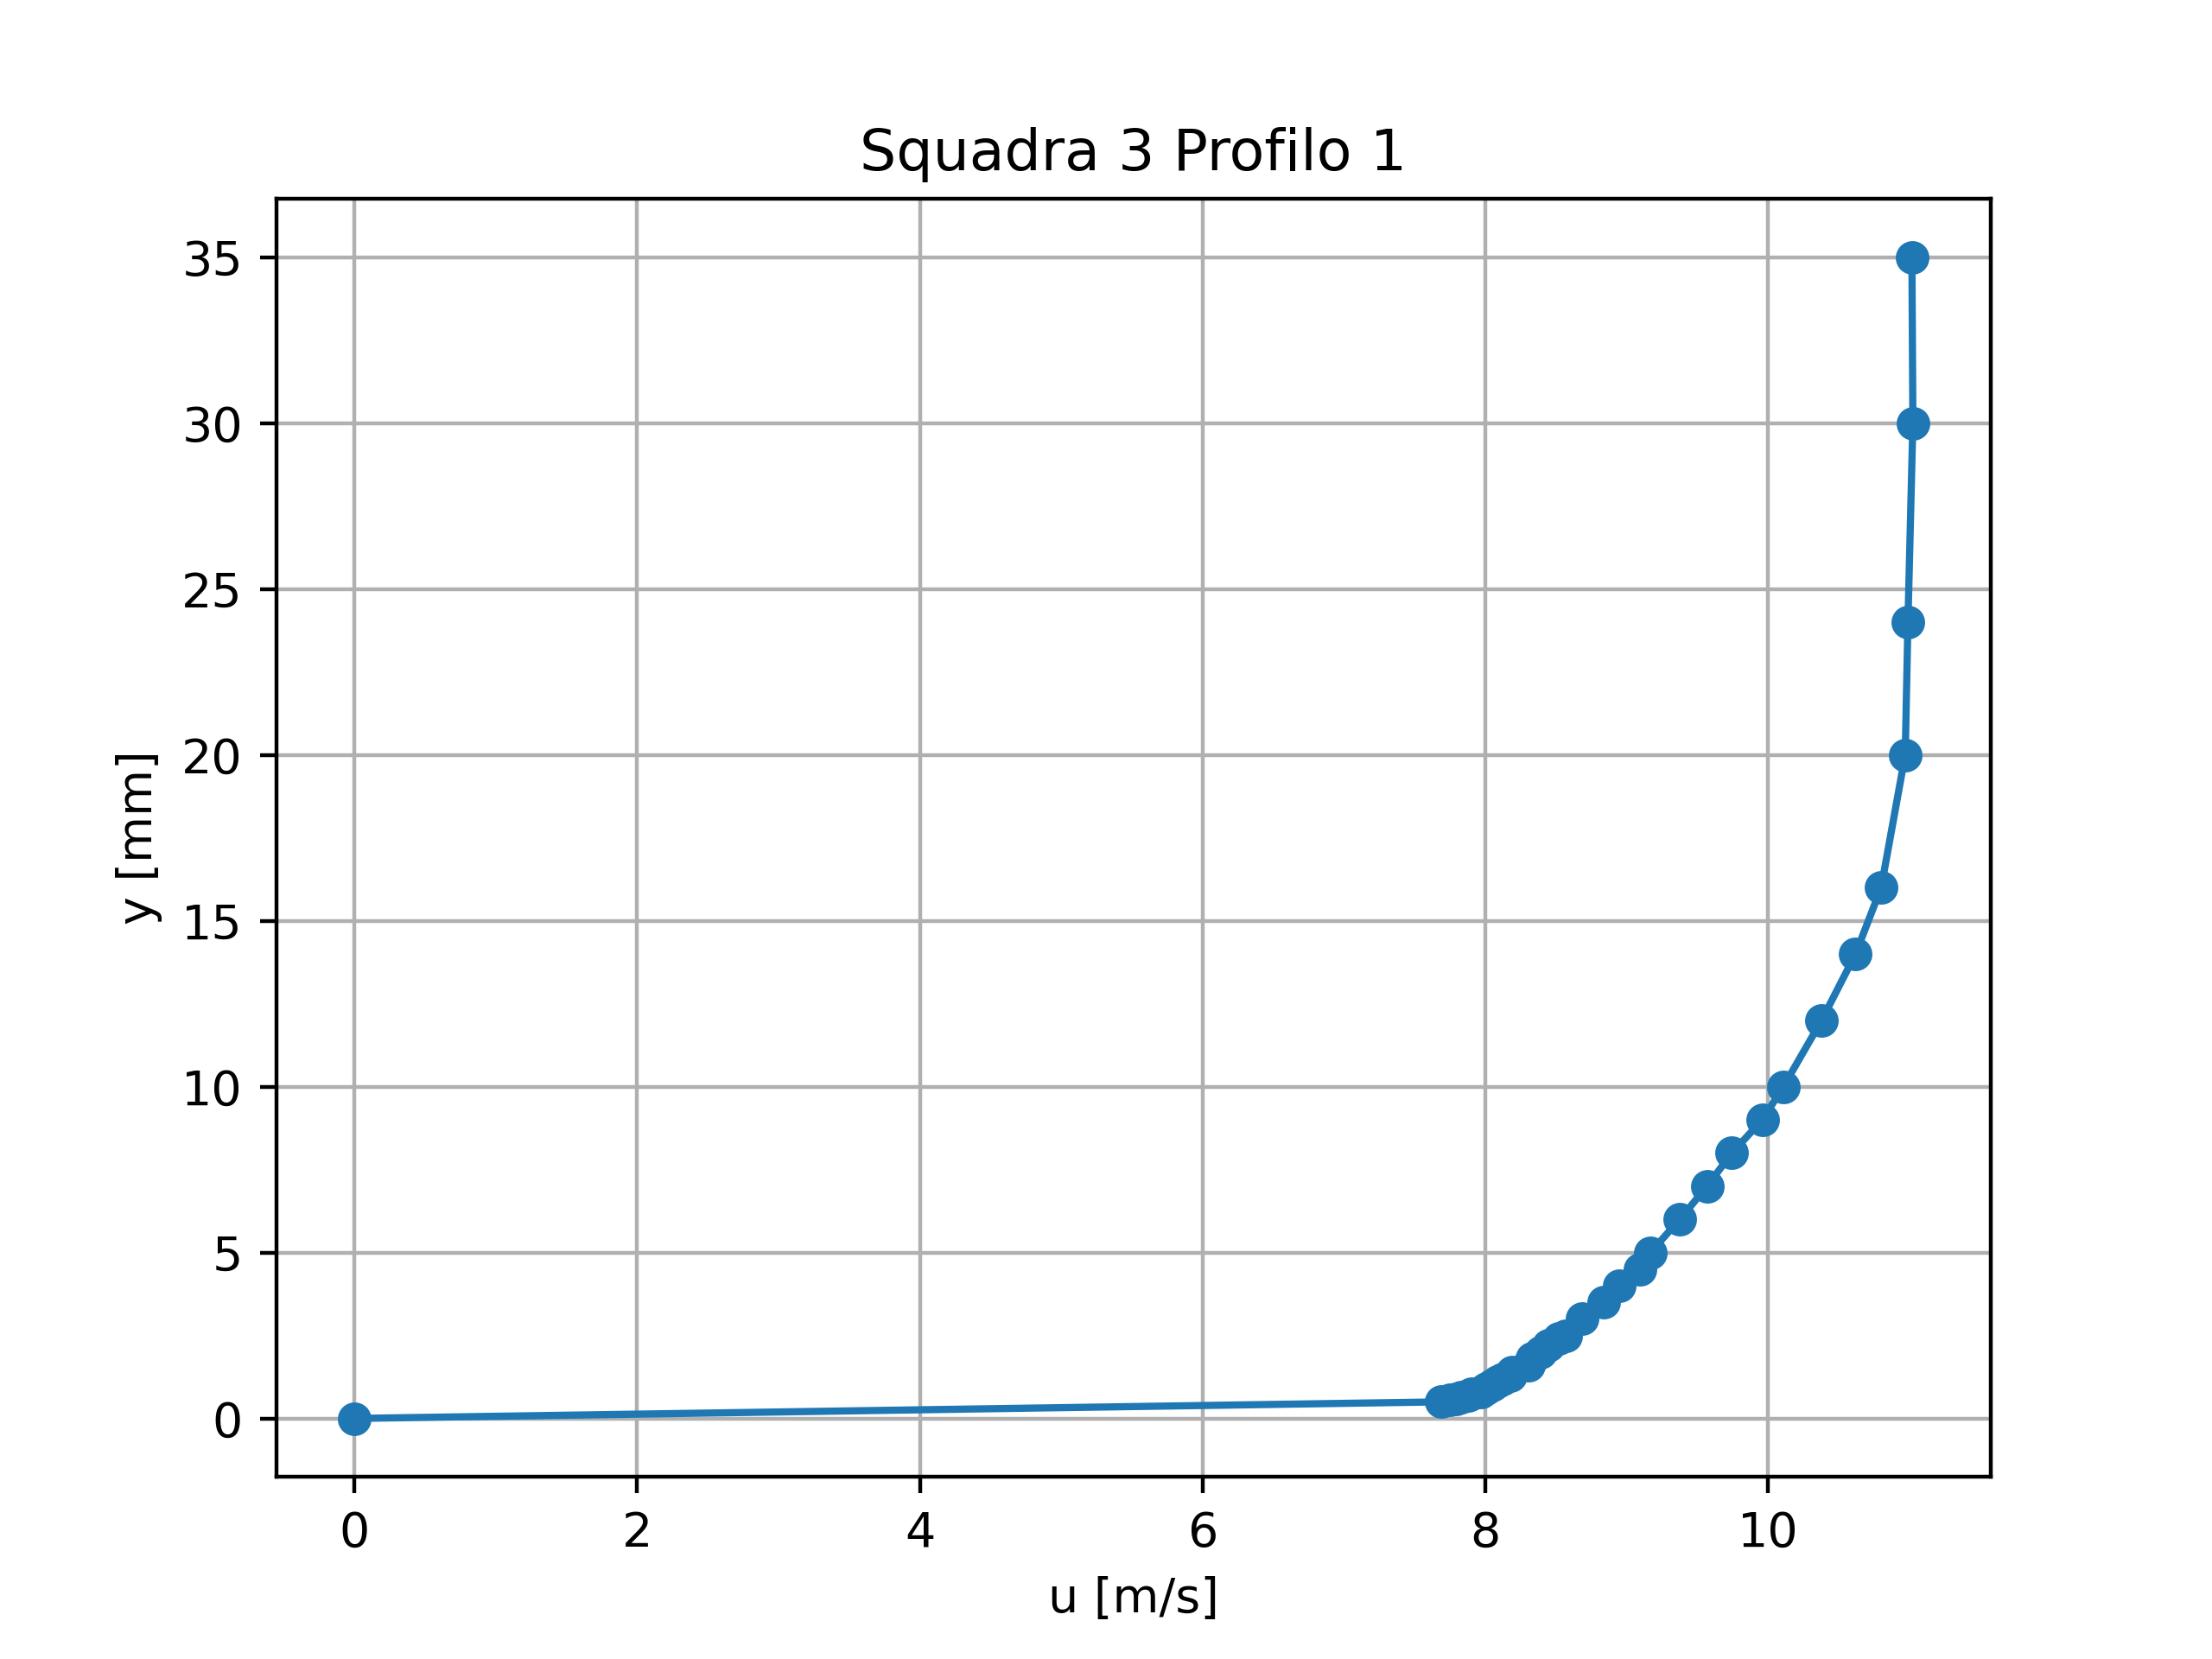
\includegraphics[width=.49\textwidth]{images/9/sq3p1.png}
    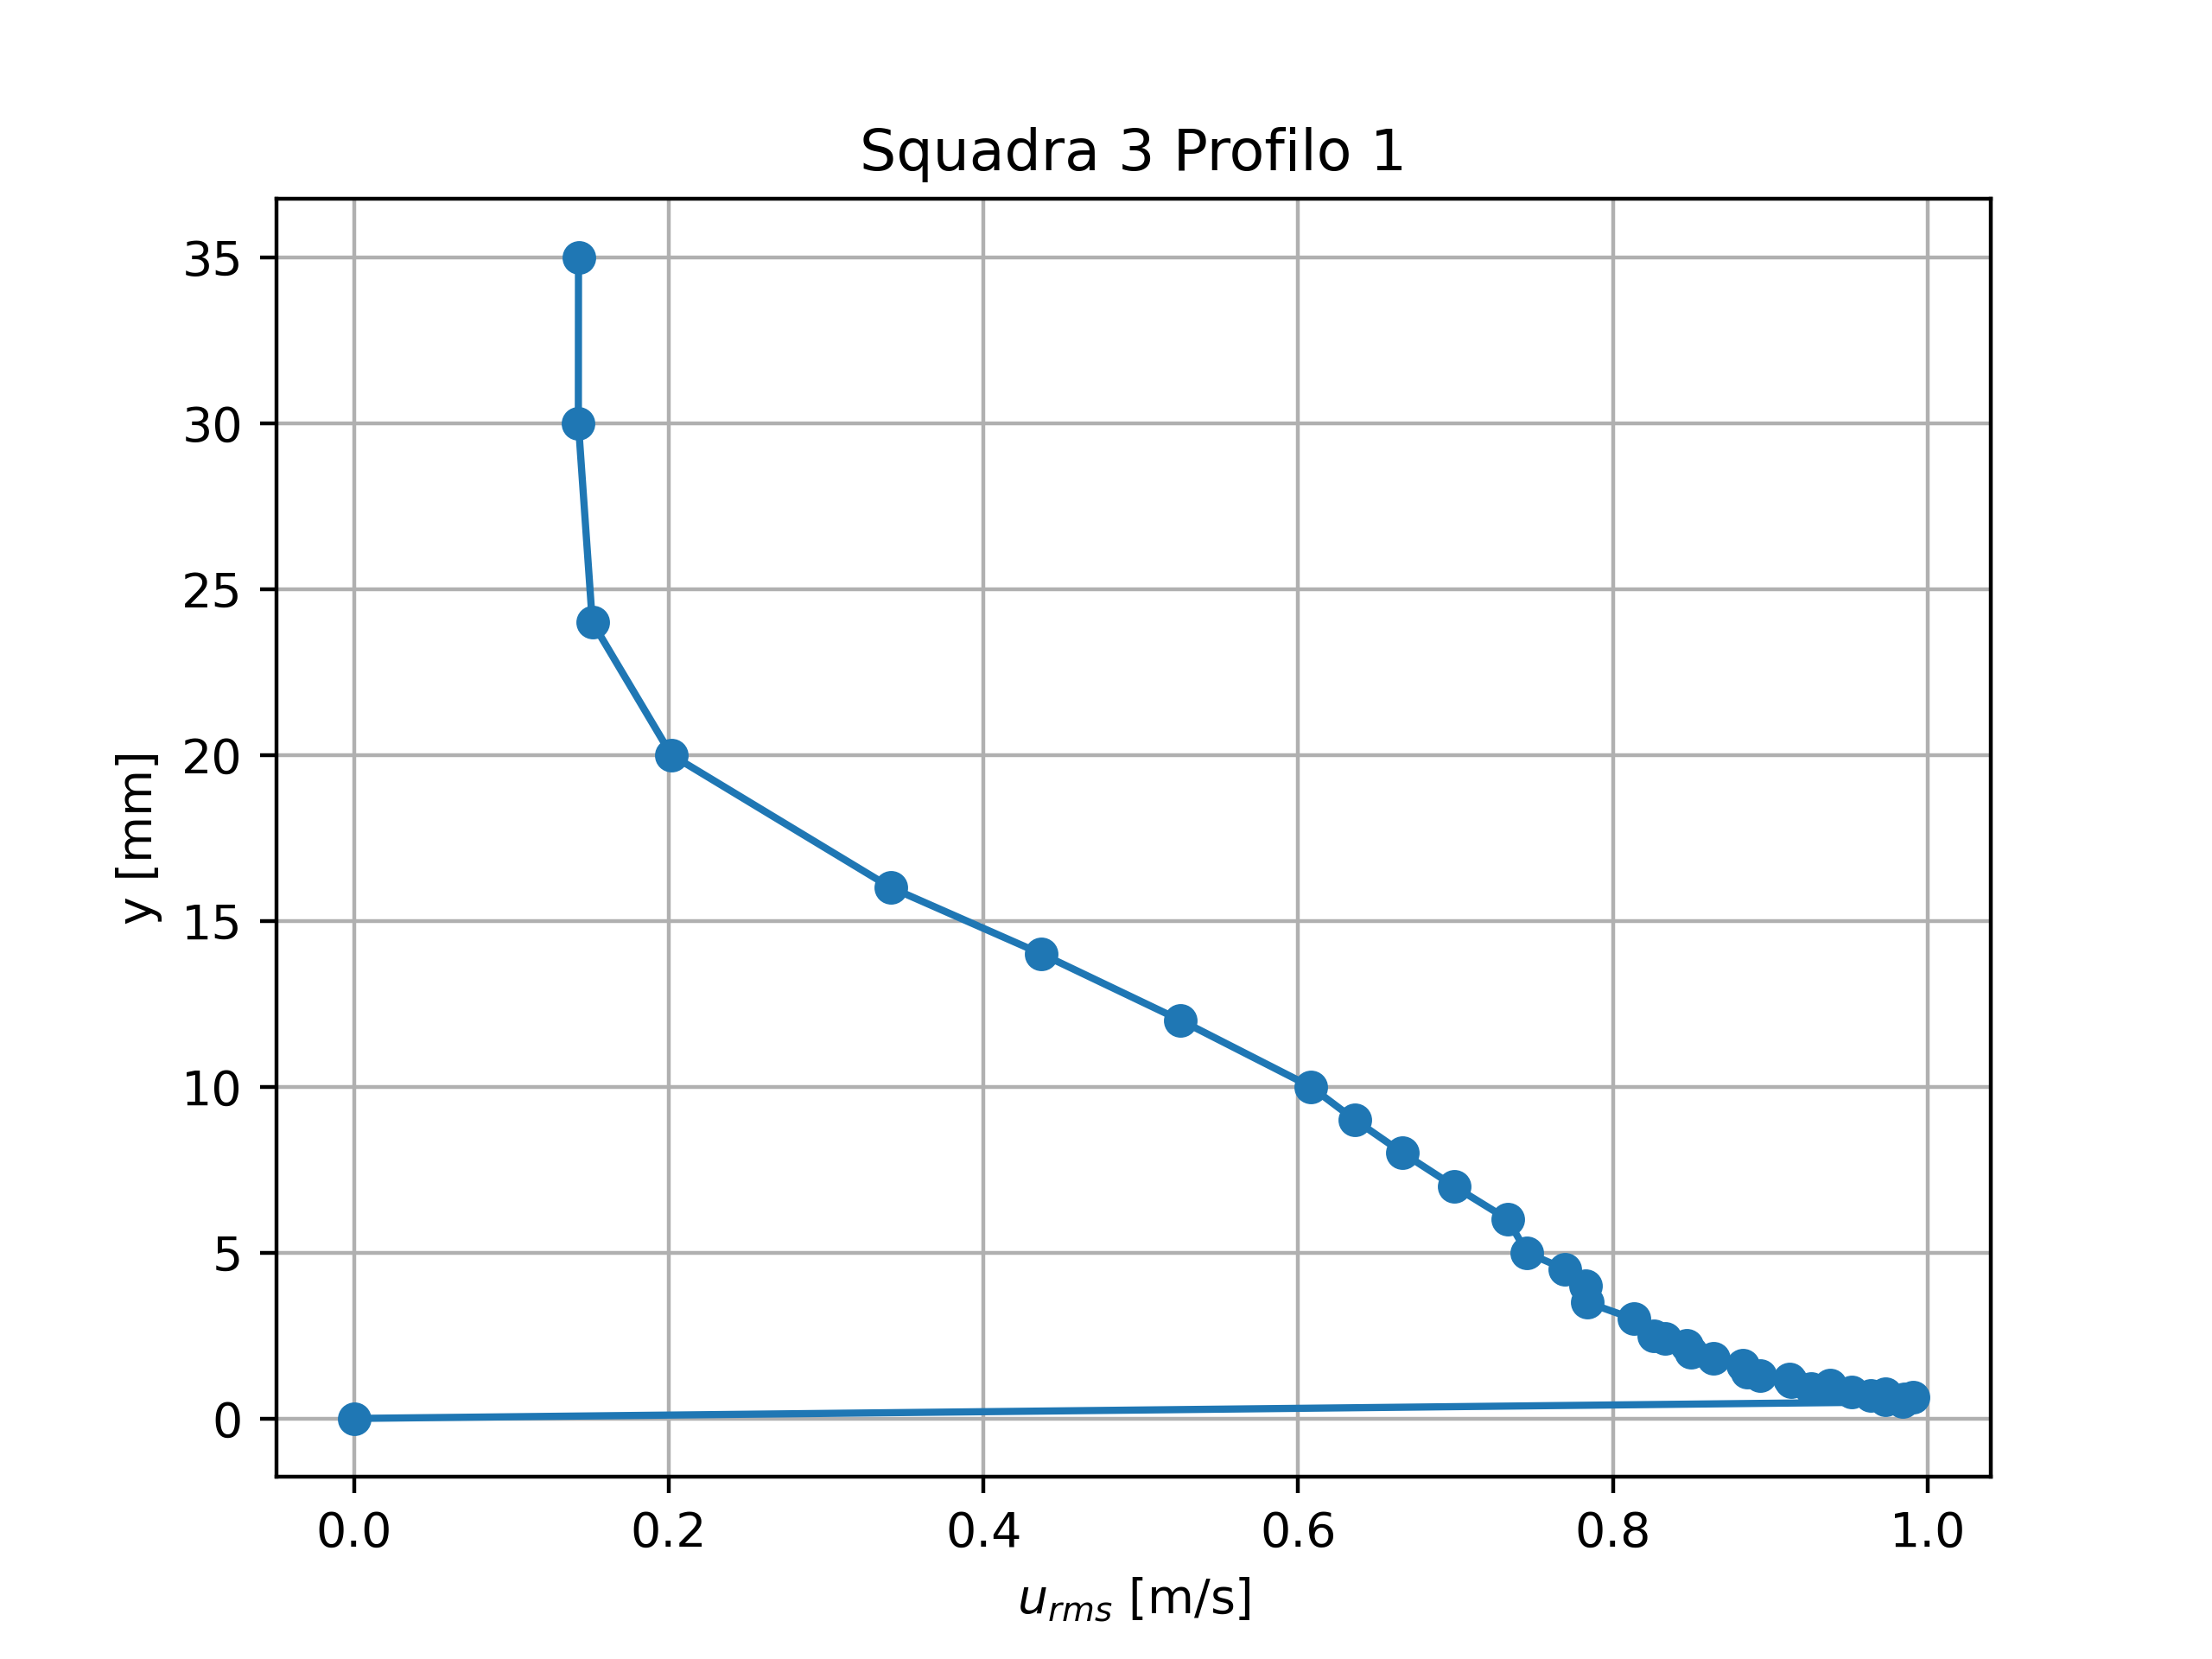
\includegraphics[width=.49\textwidth]{images/9/sq3p1rms.png}
    \caption{Esempi di profili di velocità e deviazione standard}
\end{figure}

\noindent Per stimare il valore di velocità a monte $U_\infty$, poiché per una placca piana la velocità a monte corrisponde alla velocità all'esterno dello strato limite $U_e$, si utilizzano i dati a disposizione della velocità $u(y)$, in particolare, si stima la velocità esterna dello strato limite $U_e$ come il massimo valore assunto da $u$ lungo $y$.\\\\
Mediante un'interpolazione lineare, è inoltre possibile stimare lo spessore geometrico dello strato limite $\delta(x)$, definito come la distanza da parete in cui la velocità assume il valore di $u=0.99U_e$.\\\\
Conoscendo la velocità esterna allo strato limite $U_e$ e lo spessore geometrico $\delta(x)$ è possibile diagrammare i profili di velocità in forma adimensionale $u/U_\infty=f(y/\delta)$:
\begin{figure}[H]
    \centering
    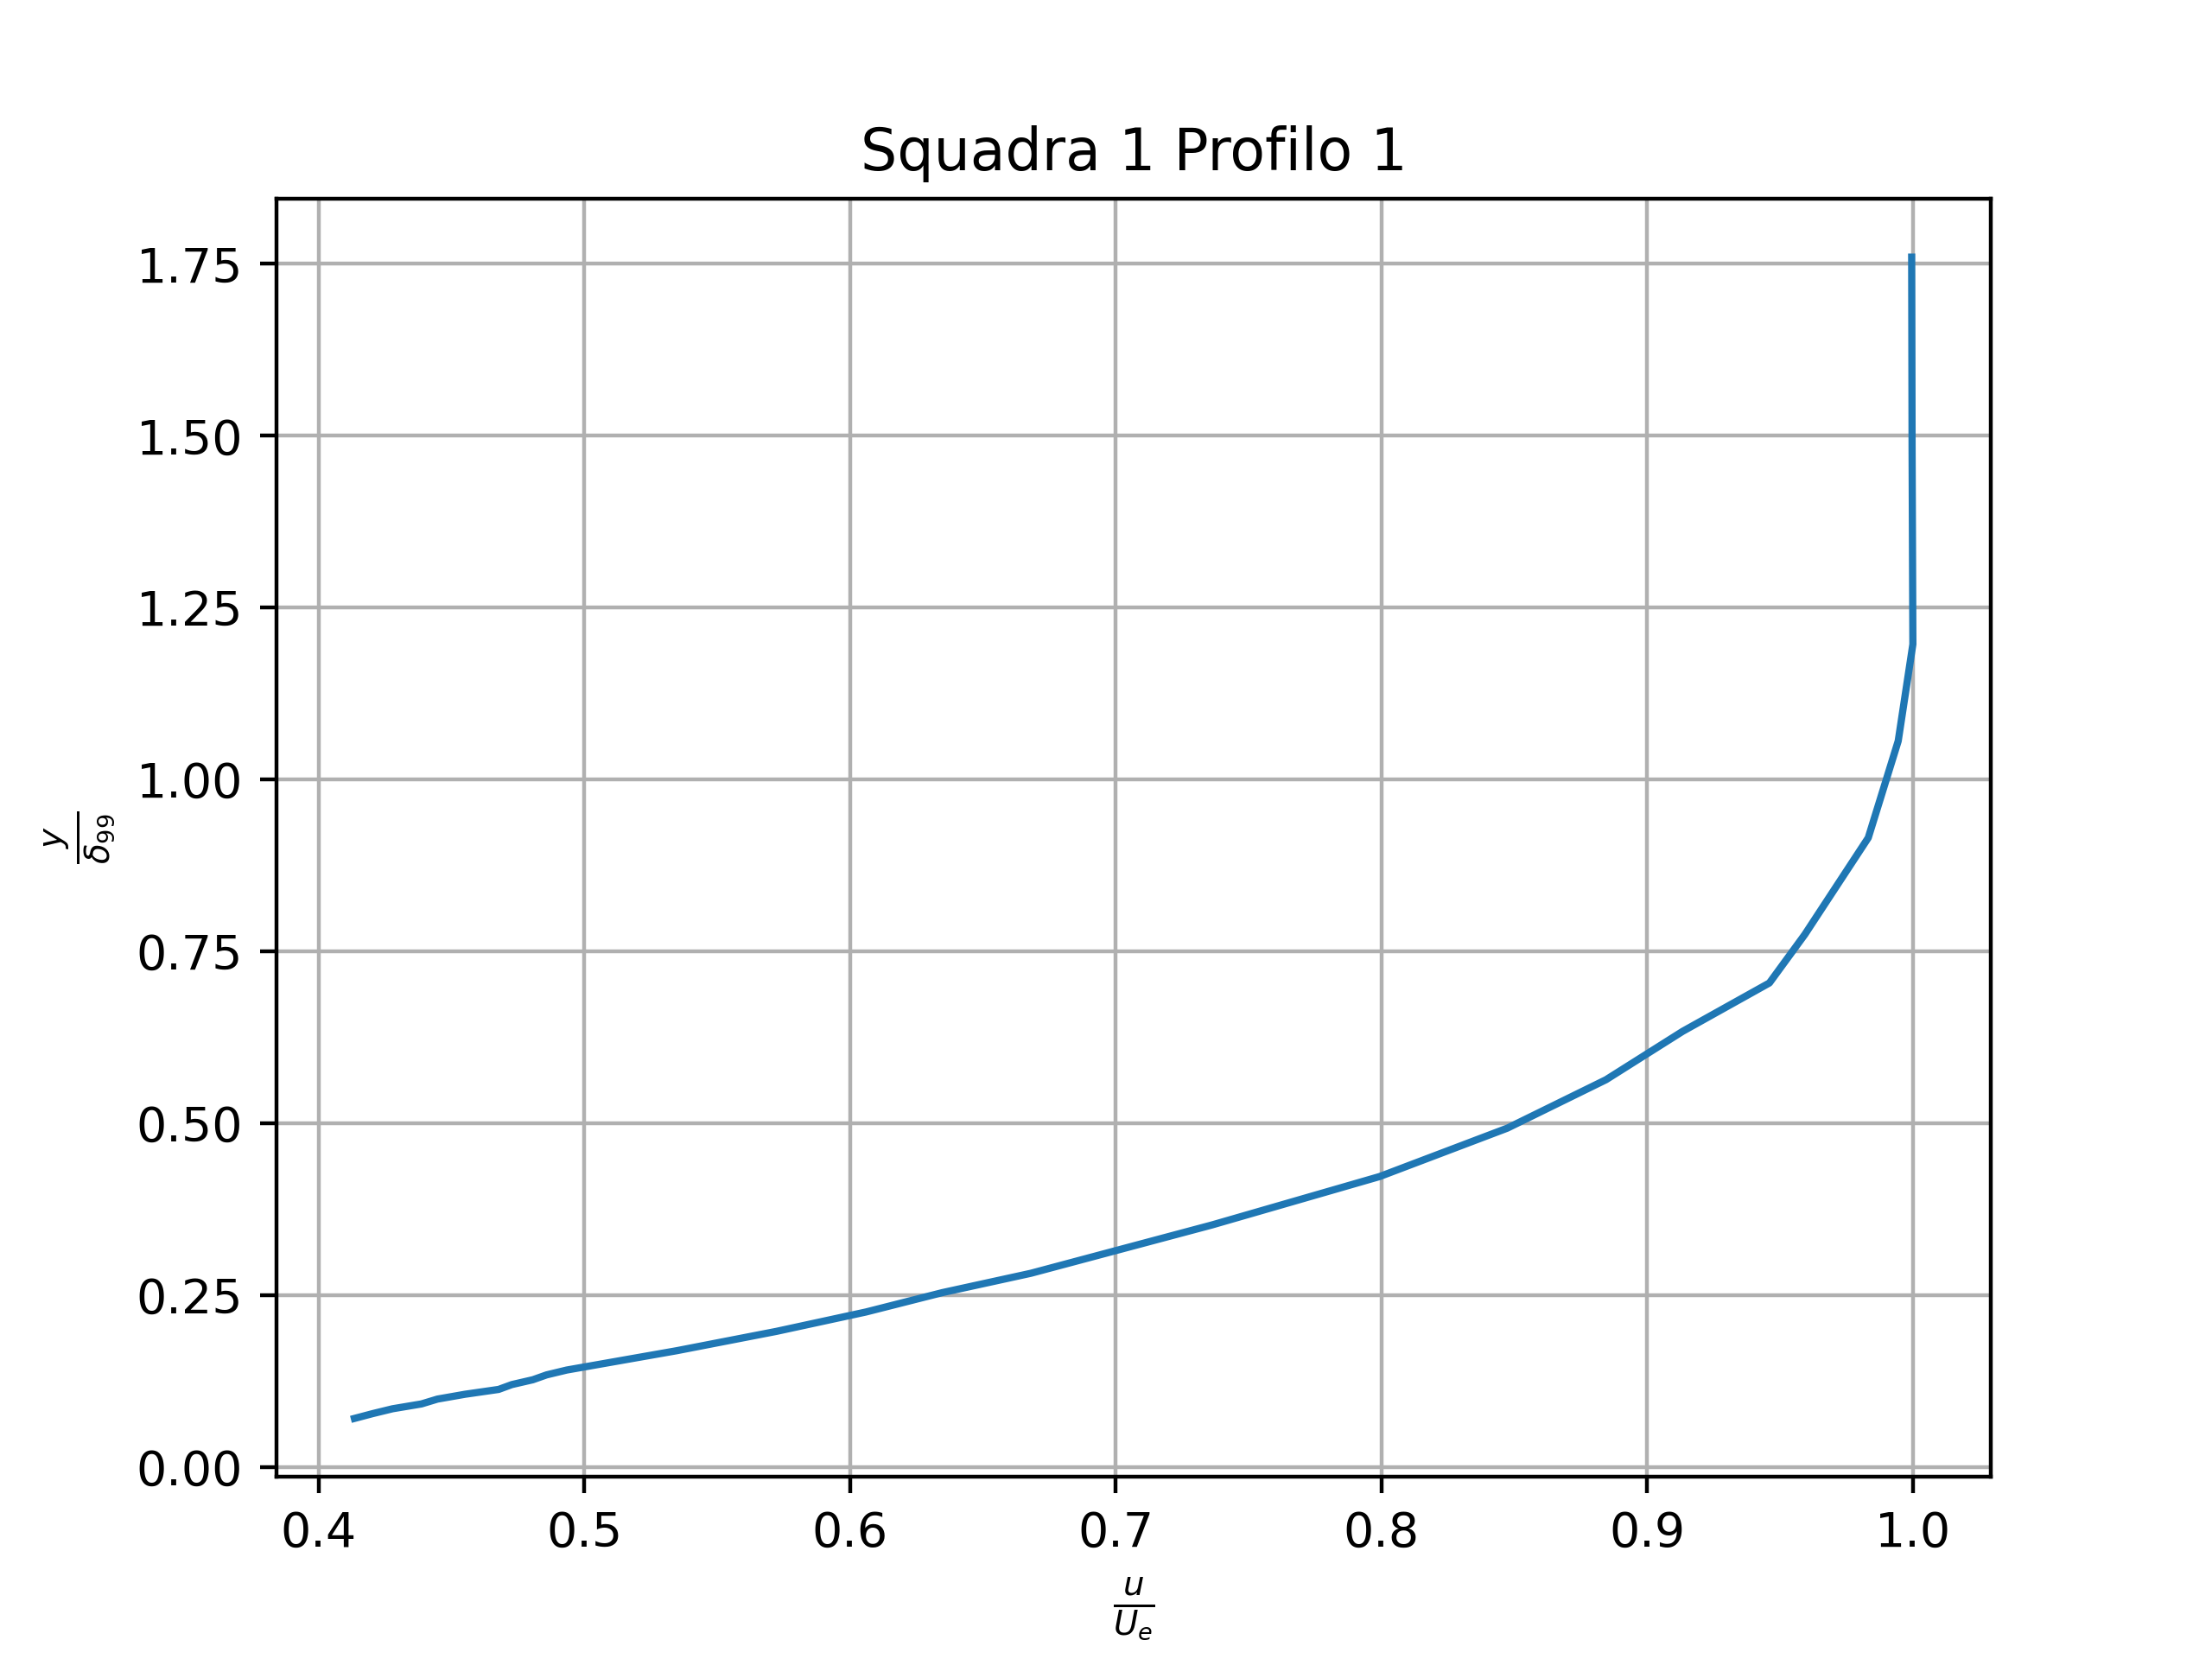
\includegraphics[width=.48\textwidth]{images/9/sq1p1_adim.png}
    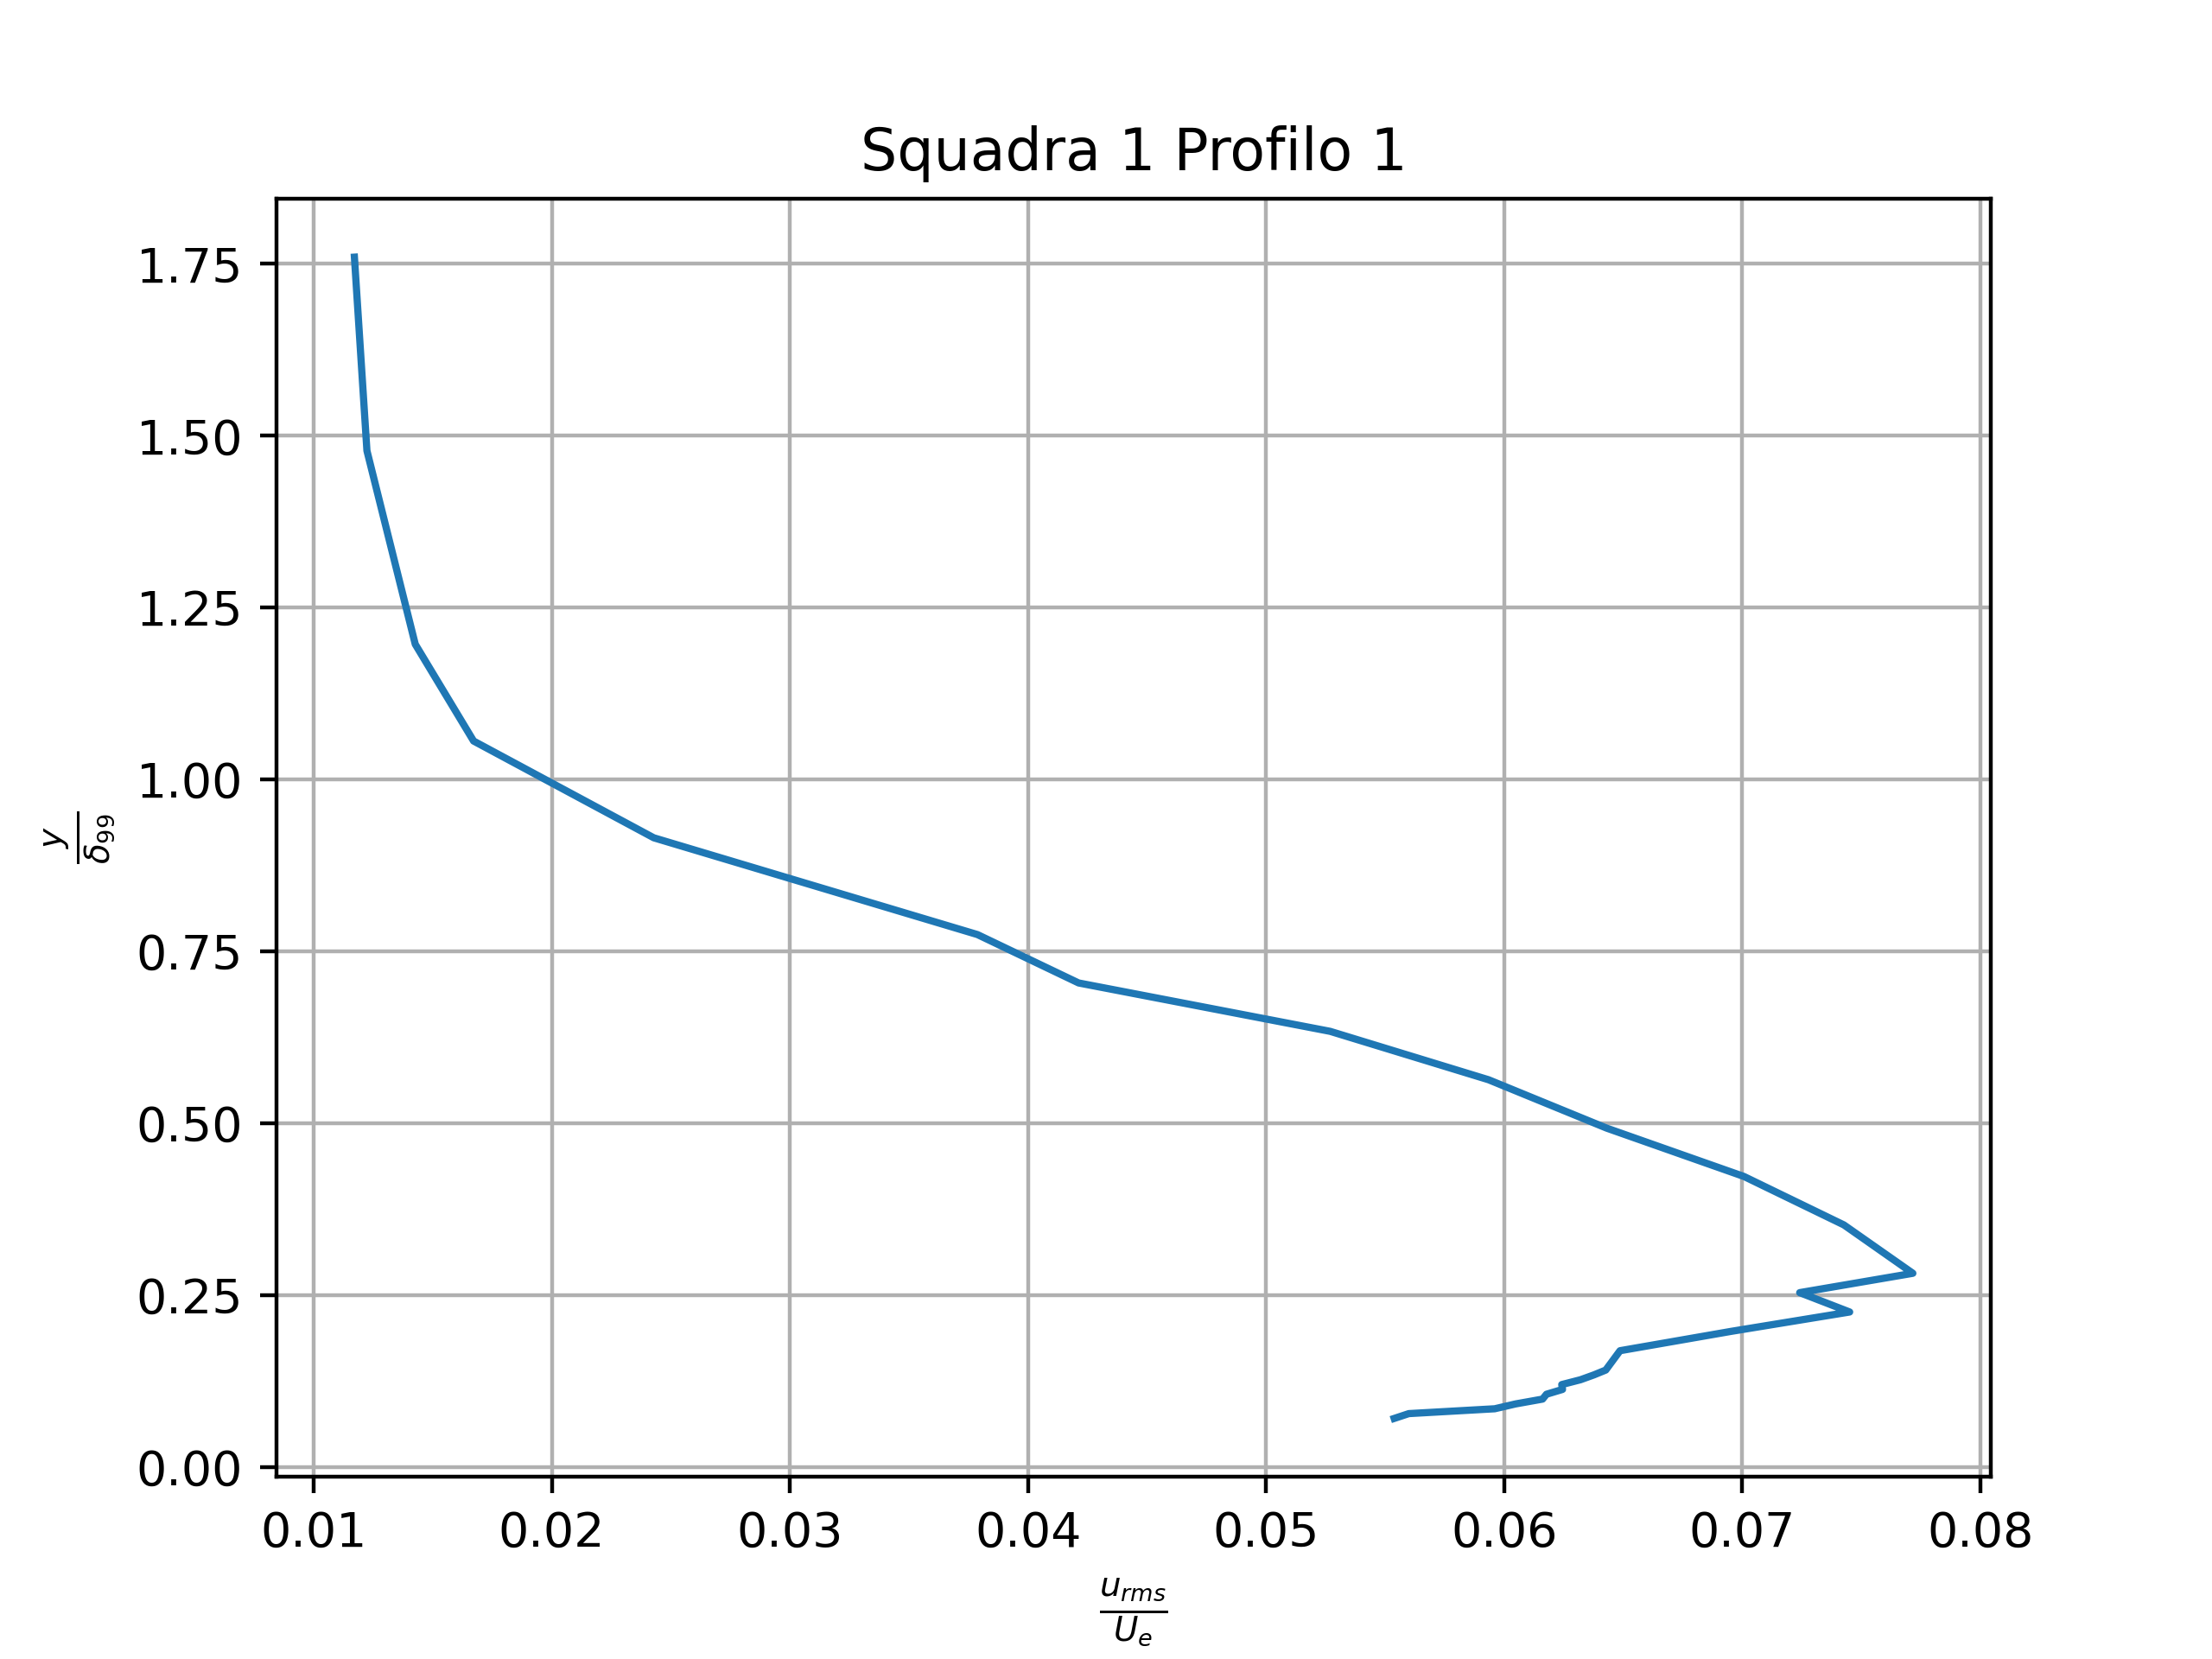
\includegraphics[width=.48\textwidth]{images/9/sq1p1_rms_adim.png}
    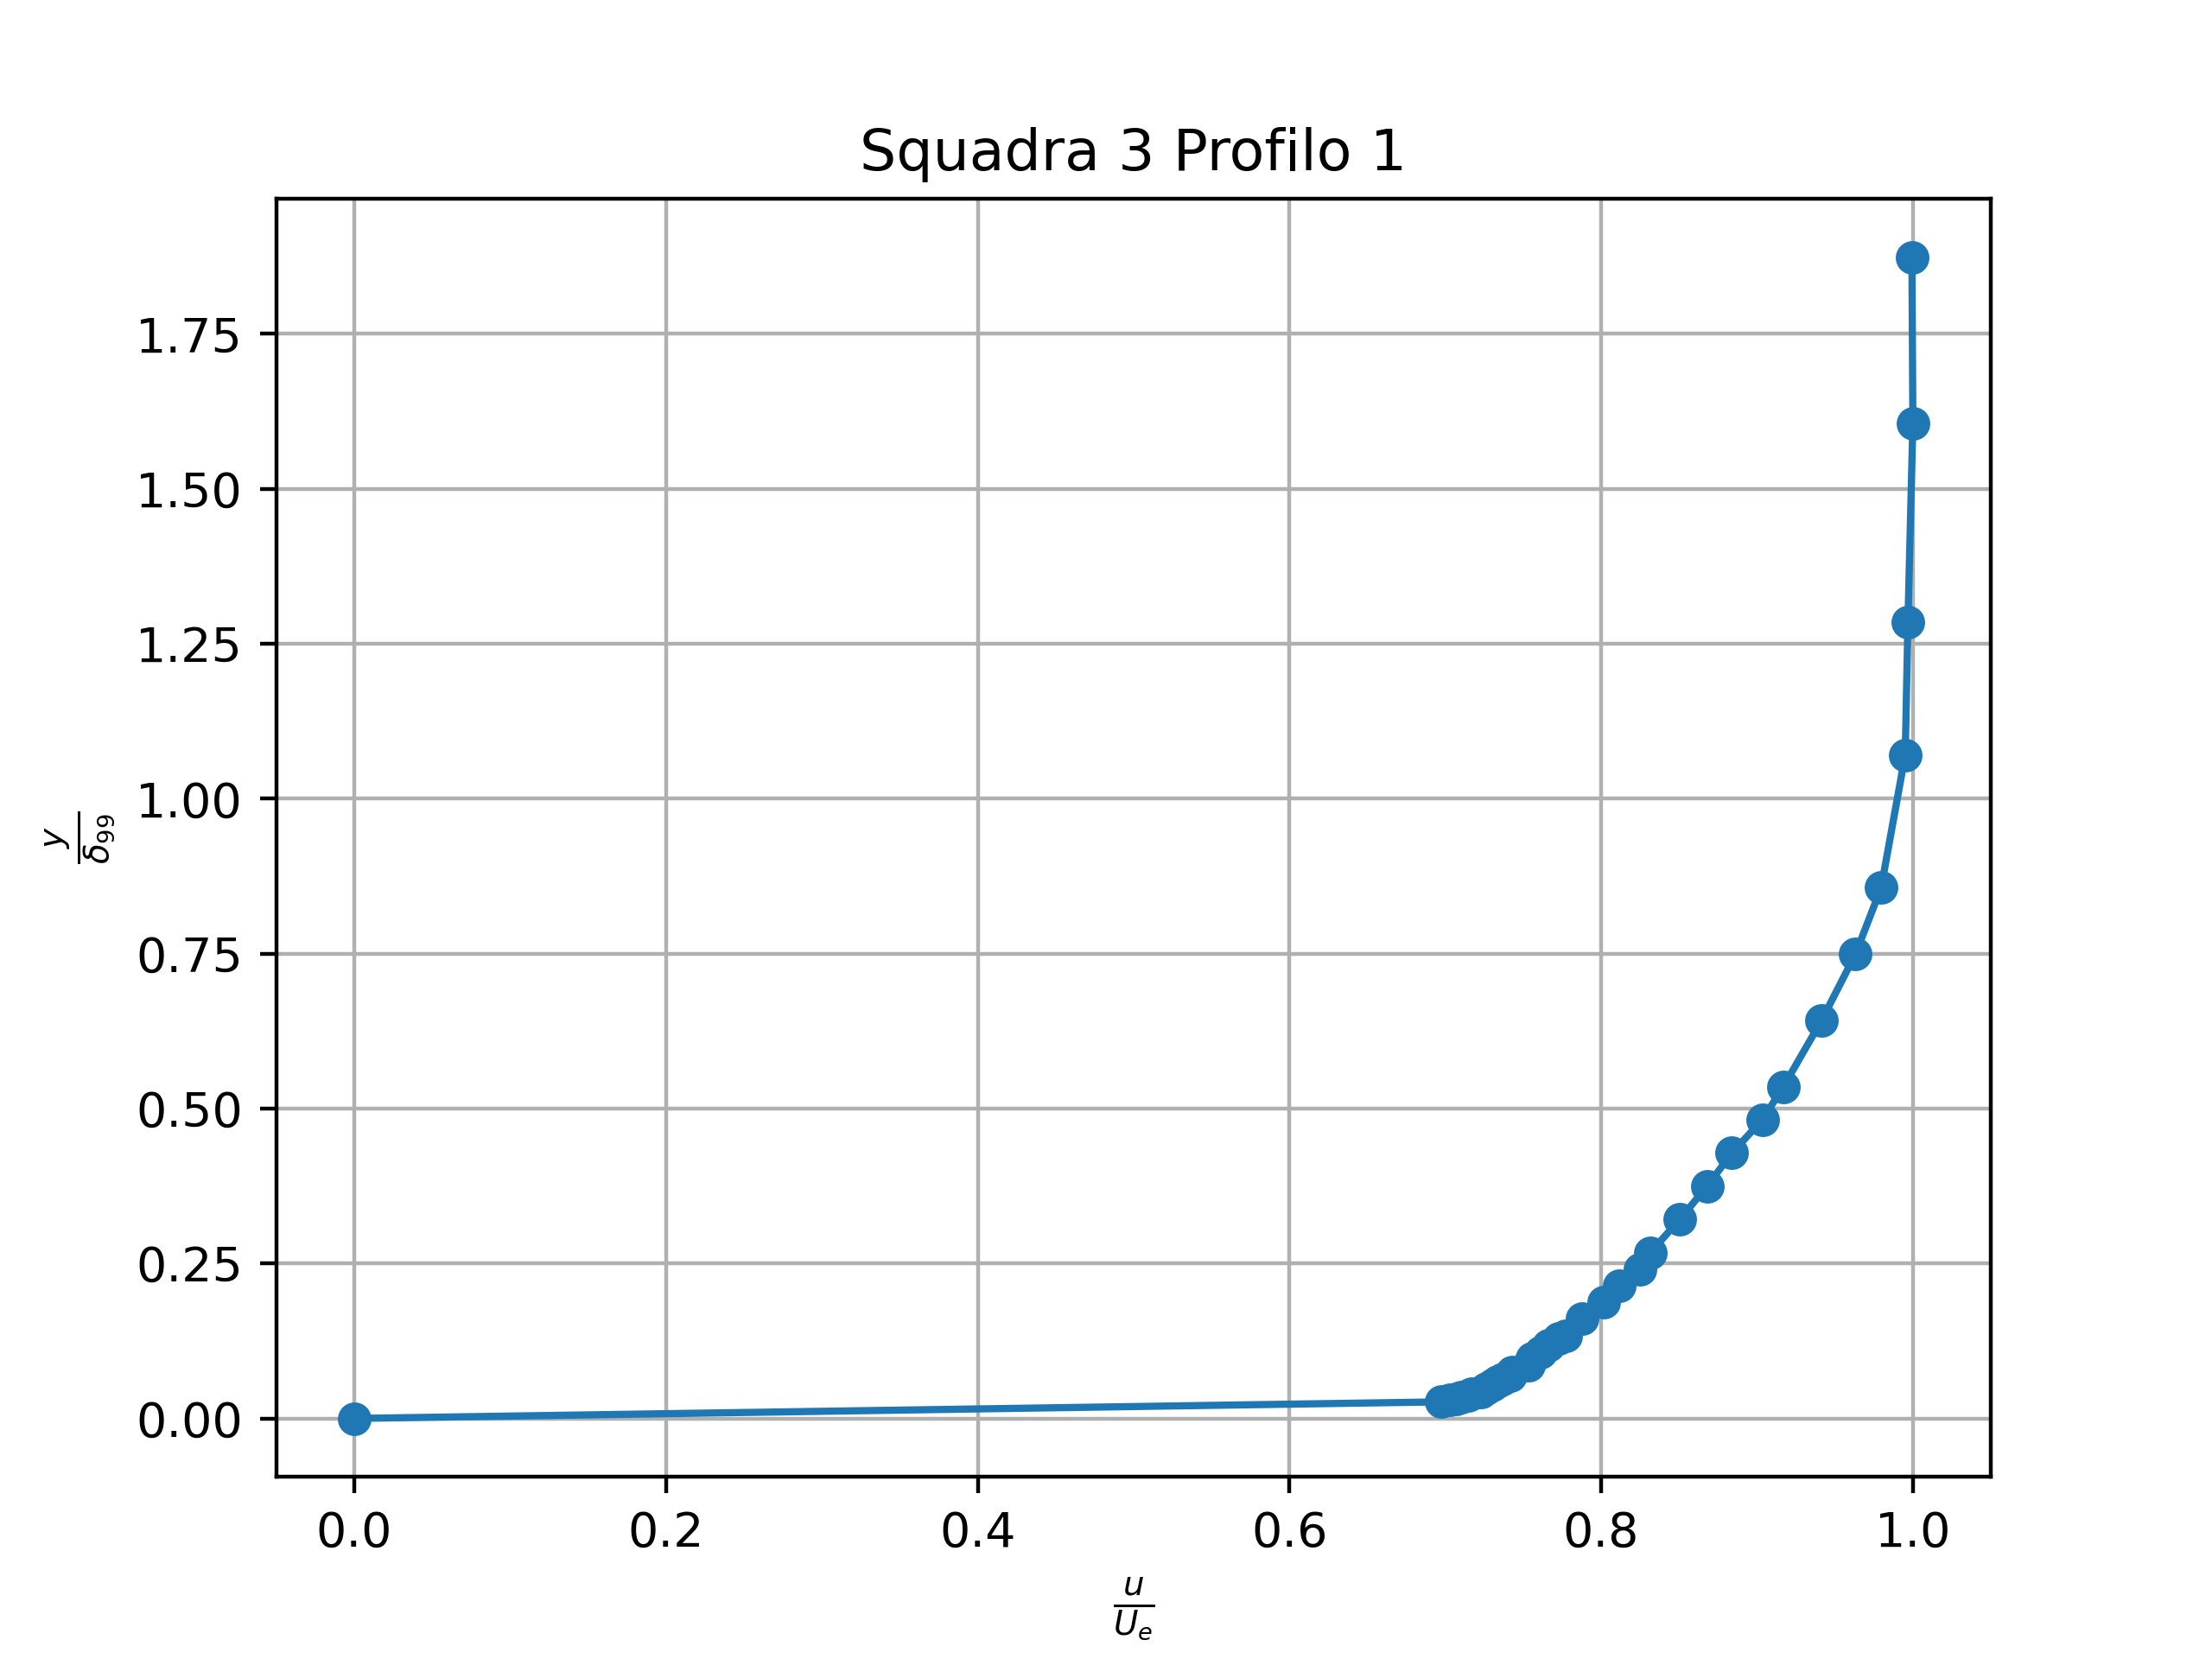
\includegraphics[width=.48\textwidth]{images/9/sq3p1_adim.png}
    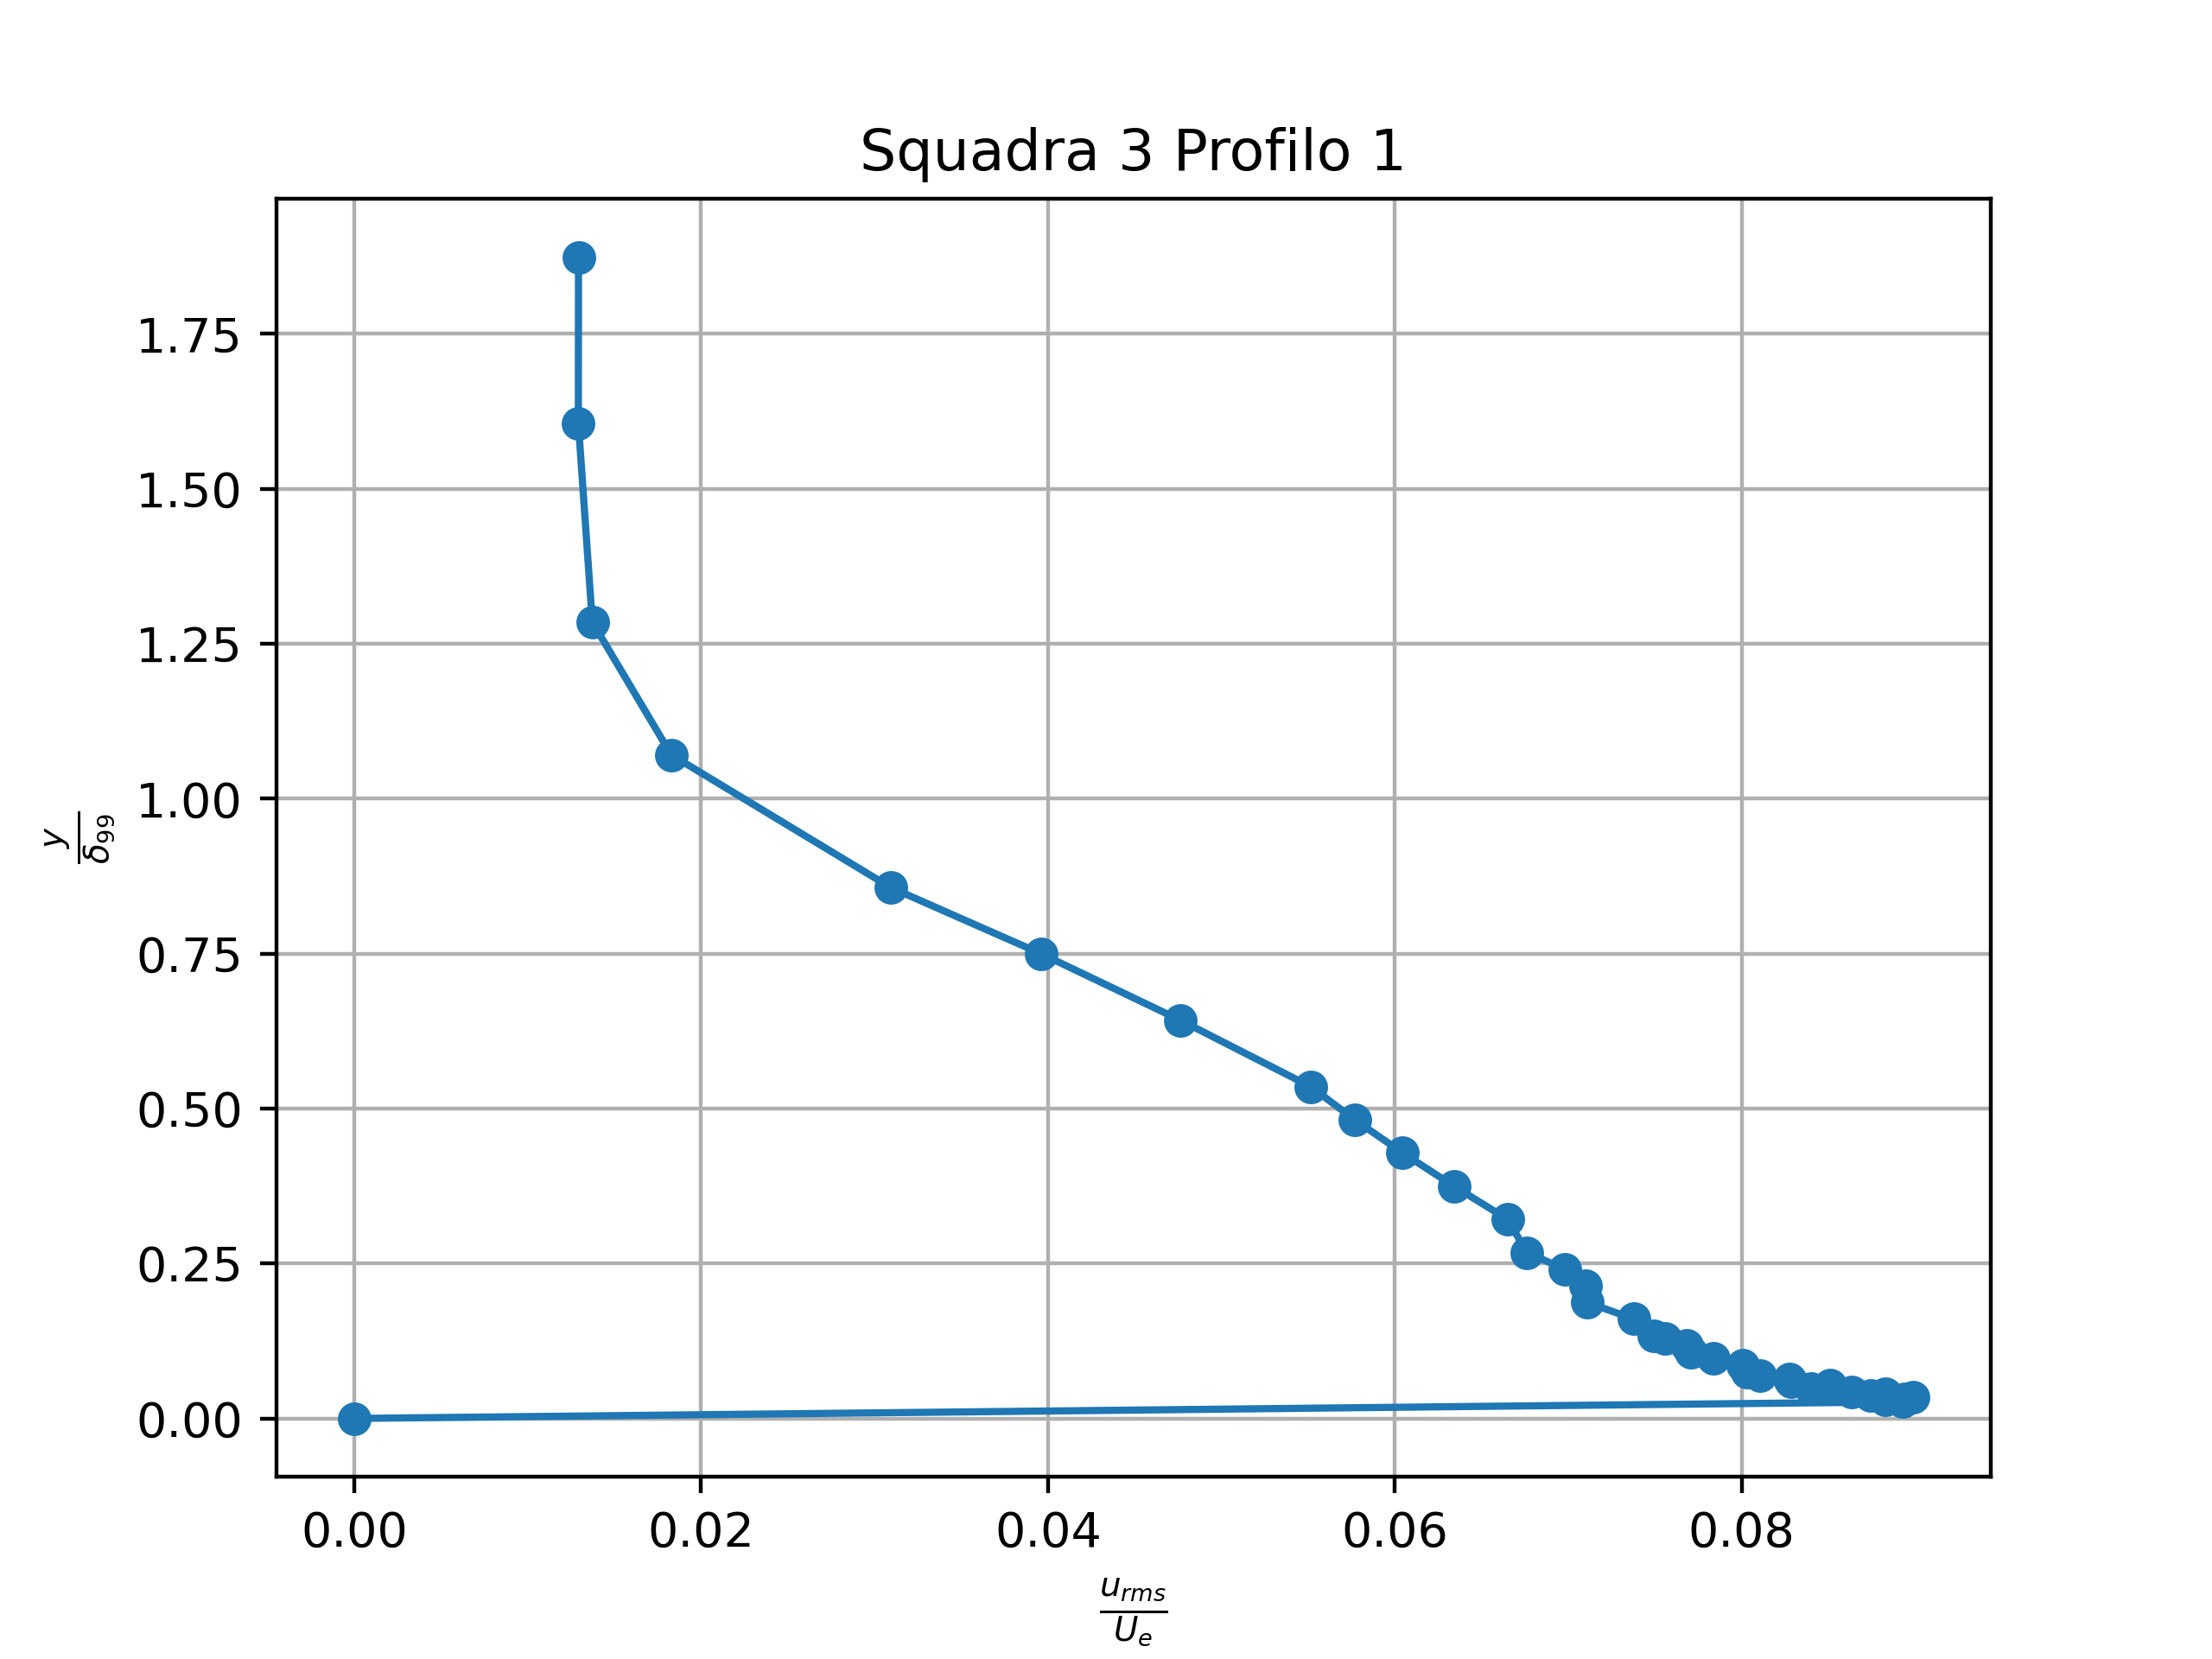
\includegraphics[width=.48\textwidth]{images/9/sq3p1_rms_adim.png}
    \caption{Esempi di profili di velocità e deviazione standard in forma adimensionale}
\end{figure}

\noindent Successivamente, si ricavano lo spessore di spostamento $\delta^*(x)$, lo spessore di quantità di moto $\theta(x)$ e il parametro di forma $H(x)$:
\begin{equation*}
    \delta^* = \int_0^\infty \left(1-\frac{u}{U_e}\right)dy \qquad \theta = \int_0^\infty \frac{u}{U_e}\left(1-\frac{u}{U_e}\right)dy \qquad H = \frac{\delta^*}{\theta}
\end{equation*}
Poiché si dispone di dati discreti, per gli integrali si utilizza la regola dei trapezi:
\begin{equation*}
    \int_a^b f(x)dx \approx \sum_{k=1}^n \frac{f(x_{k-1}) + f(x_k)}2 \Delta x_k \quad \text{con } \Delta x_k = x_k - x_{k-1}
\end{equation*}
Per metodo più immmediato per determinare se lo strato limite analizzato è laminare, transizionale o turbolento, è il calcolod del numero di Reynolds locale $Re_x$, relativo alla coordinata $x$, se questo è maggiore del numero di Reynolds critico ($Re_{cr}\approx500000$) allora lo strato limite è laminare, altrimenti è turbolento:
\begin{equation*}
    Re_x = \frac{U_\infty x}\nu
\end{equation*}
Per le otto configurazioni, si ottengono i seguenti risultati:\\\\
\textbf{Squadra 1}\\
$-$ Profilo 1: $Re_x=316408\ \rightarrow\ $ strato limite laminare;\\
$-$ Profilo 2: $Re_x=521112\ \rightarrow\ $ strato limite turbolento;\\\\
\textbf{Squadra 2}\\
$-$ Profilo 1: $Re_x=358159\ \rightarrow\ $ strato limite laminare;\\
$-$ Profilo 2: $Re_x=649986\ \rightarrow\ $ strato limite turbolento;\\\\
\textbf{Squadra 3}\\
$-$ Profilo 1: $Re_x=656506\ \rightarrow\ $ strato limite turbolento;\\
$-$ Profilo 2: $Re_x=214079\ \rightarrow\ $ strato limite laminare;\\\\
\textbf{Squadra 4}\\
$-$ Profilo 1: $Re_x=143967\ \rightarrow\ $ strato limite laminare;\\
$-$ Profilo 2: $Re_x=498714\ \rightarrow\ $ strato limite transizionale;\\\\
Un altro parametro utile a determinare il regime dello strato limite è il parametro di forma $H(x)$. Questo infatti assume un valore $H\approx2.59$ (soluzione di Blasius) nel caso di strato limite laminare, mentre assume un valore attorno a $H\approx1.3$ nel caso di strato limite turbolento.\\\\
Si ottengono i seguenti risultati per le grandezze caratteristiche dello strato limite per le otto configurazioni: 
\begin{table}[H]
    \centering
    \begin{tabular}{|c|c|c|c|c|c|}
    \hline
    Configurazione             & $Re_x$ & $\delta_{99}$ & $\delta^*$ & $\theta$ & $H$  \\ \hline
    Squadra 1 Profilo 1 & 316408 & 7.10 mm     & 1.26 mm    & 0.83 mm  & 1.52 \\ \hline
    Squadra 1 Profilo 2 & 521112 & 21.19 mm    & 2.07 mm    & 1.72 mm  & 1.20 \\ \hline
    Squadra 2 Profilo 1 & 358159 & 6.53 mm     & 1.53 mm    & 0.79 mm  & 1.92 \\ \hline
    Squadra 2 Profilo 2 & 649986 & 21.17 mm    & 2.45 mm    & 1.81 mm  & 1.35 \\ \hline
    Squadra 3 Profilo 1 & 656506 & 18.68 mm    & 2.31 mm    & 1.72 mm  & 1.35 \\ \hline
    Squadra 3 Profilo 2 & 214079 & 15.81 mm    & 3.93 mm    & 1.96 mm  & 2.01 \\ \hline
    Squadra 4 Profilo 1 & 143967 & 17.17 mm    & 5.11 mm    & 2.06 mm  & 2.48 \\ \hline
    Squadra 4 Profilo 2 & 498714 & 13.50 mm    & 1.96 mm    & 1.32 mm  & 1.48 \\ \hline
    \end{tabular}
\end{table}

\noindent Si evince che il parametro di forma in alcune configurazioni non rispetta la considerazione teorica precedentemente espressa. Questo è dovuto al fatto che in alcune configurazioni lo strato limite è transizionale, e presenta pertanto turbolenza intermittente. Si osserva inoltre come lo spessore geometrico $\delta_{99}$ dello strato limite sia fortemente influenzato dalla distanza $x$ dal bordo di attacco della placca piana (lo spessore dello strato limite aumenta lungo la placca piana).\\\\
\noindent È opportuno confrontare i risultati ottenuti con i risultati empirici previsti dalla teoria:
\begin{table}[H]
    \centering
    \begin{tabular}{|c|c|c|c|c|c|}
    \hline
    Configurazione             & $Re_x$ & $\delta_{99,emp}$ & $\delta^*_{emp}$ & $\theta_{emp}$ & $H_{emp}$ \\ \hline
    Squadra 1 Profilo 1 & 316408 & 4.89 mm           & 1.69 mm          & 0.65 mm        & 2.61      \\ \hline
    Squadra 1 Profilo 2 & 521112 & 23.94 mm          & 2.99 mm          & 2.33 mm        & 1.28      \\ \hline
    Squadra 2 Profilo 1 & 358159 & 4.18 mm           & 1.45 mm          & 0.55 mm        & 2.61      \\ \hline
    Squadra 2 Profilo 2 & 649986 & 22.90 mm          & 2.86 mm          & 2.23 mm        & 1.28      \\ \hline
    Squadra 3 Profilo 1 & 656506 & 22.86 mm          & 2.86 mm          & 2.22 mm        & 1.28      \\ \hline
    Squadra 3 Profilo 2 & 214079 & 9.73 mm           & 3.37 mm          & 1.29 mm        & 2.61      \\ \hline
    Squadra 4 Profilo 1 & 143967 & 9.22 mm           & 3.19 mm          & 1.22 mm        & 2.61      \\ \hline
    Squadra 4 Profilo 2 & 498714 & 18.78 mm          & 2.35 mm          & 1.83 mm        & 1.28      \\ \hline
    \end{tabular}
\end{table}

\noindent Come già accennato, i dati risultanti delle formulazioni empiriche per alcune configurazioni si discostano dai risultati sperimentali per via del regime transizionale dello strato limite.\\\\
Nel caso di strato limite laminare la soluzione delle equazioni porta alla soluzione esatta di Blasius, che definisce il profilo di velocità in forma adimensionale:
\begin{equation*}
    \eta(x,y) \approx \frac{y}{\delta(x)} = y\sqrt{\frac{U_\infty}{\nu x}} \qquad f^\prime = \frac{u}{V_\infty}
\end{equation*}
È opportuno confrontare la teoria di Blasius con i risultati sperimentali ottenuti. Si ottengono quindi i seguenti diagrammi:
\begin{figure}[H]
    \centering
    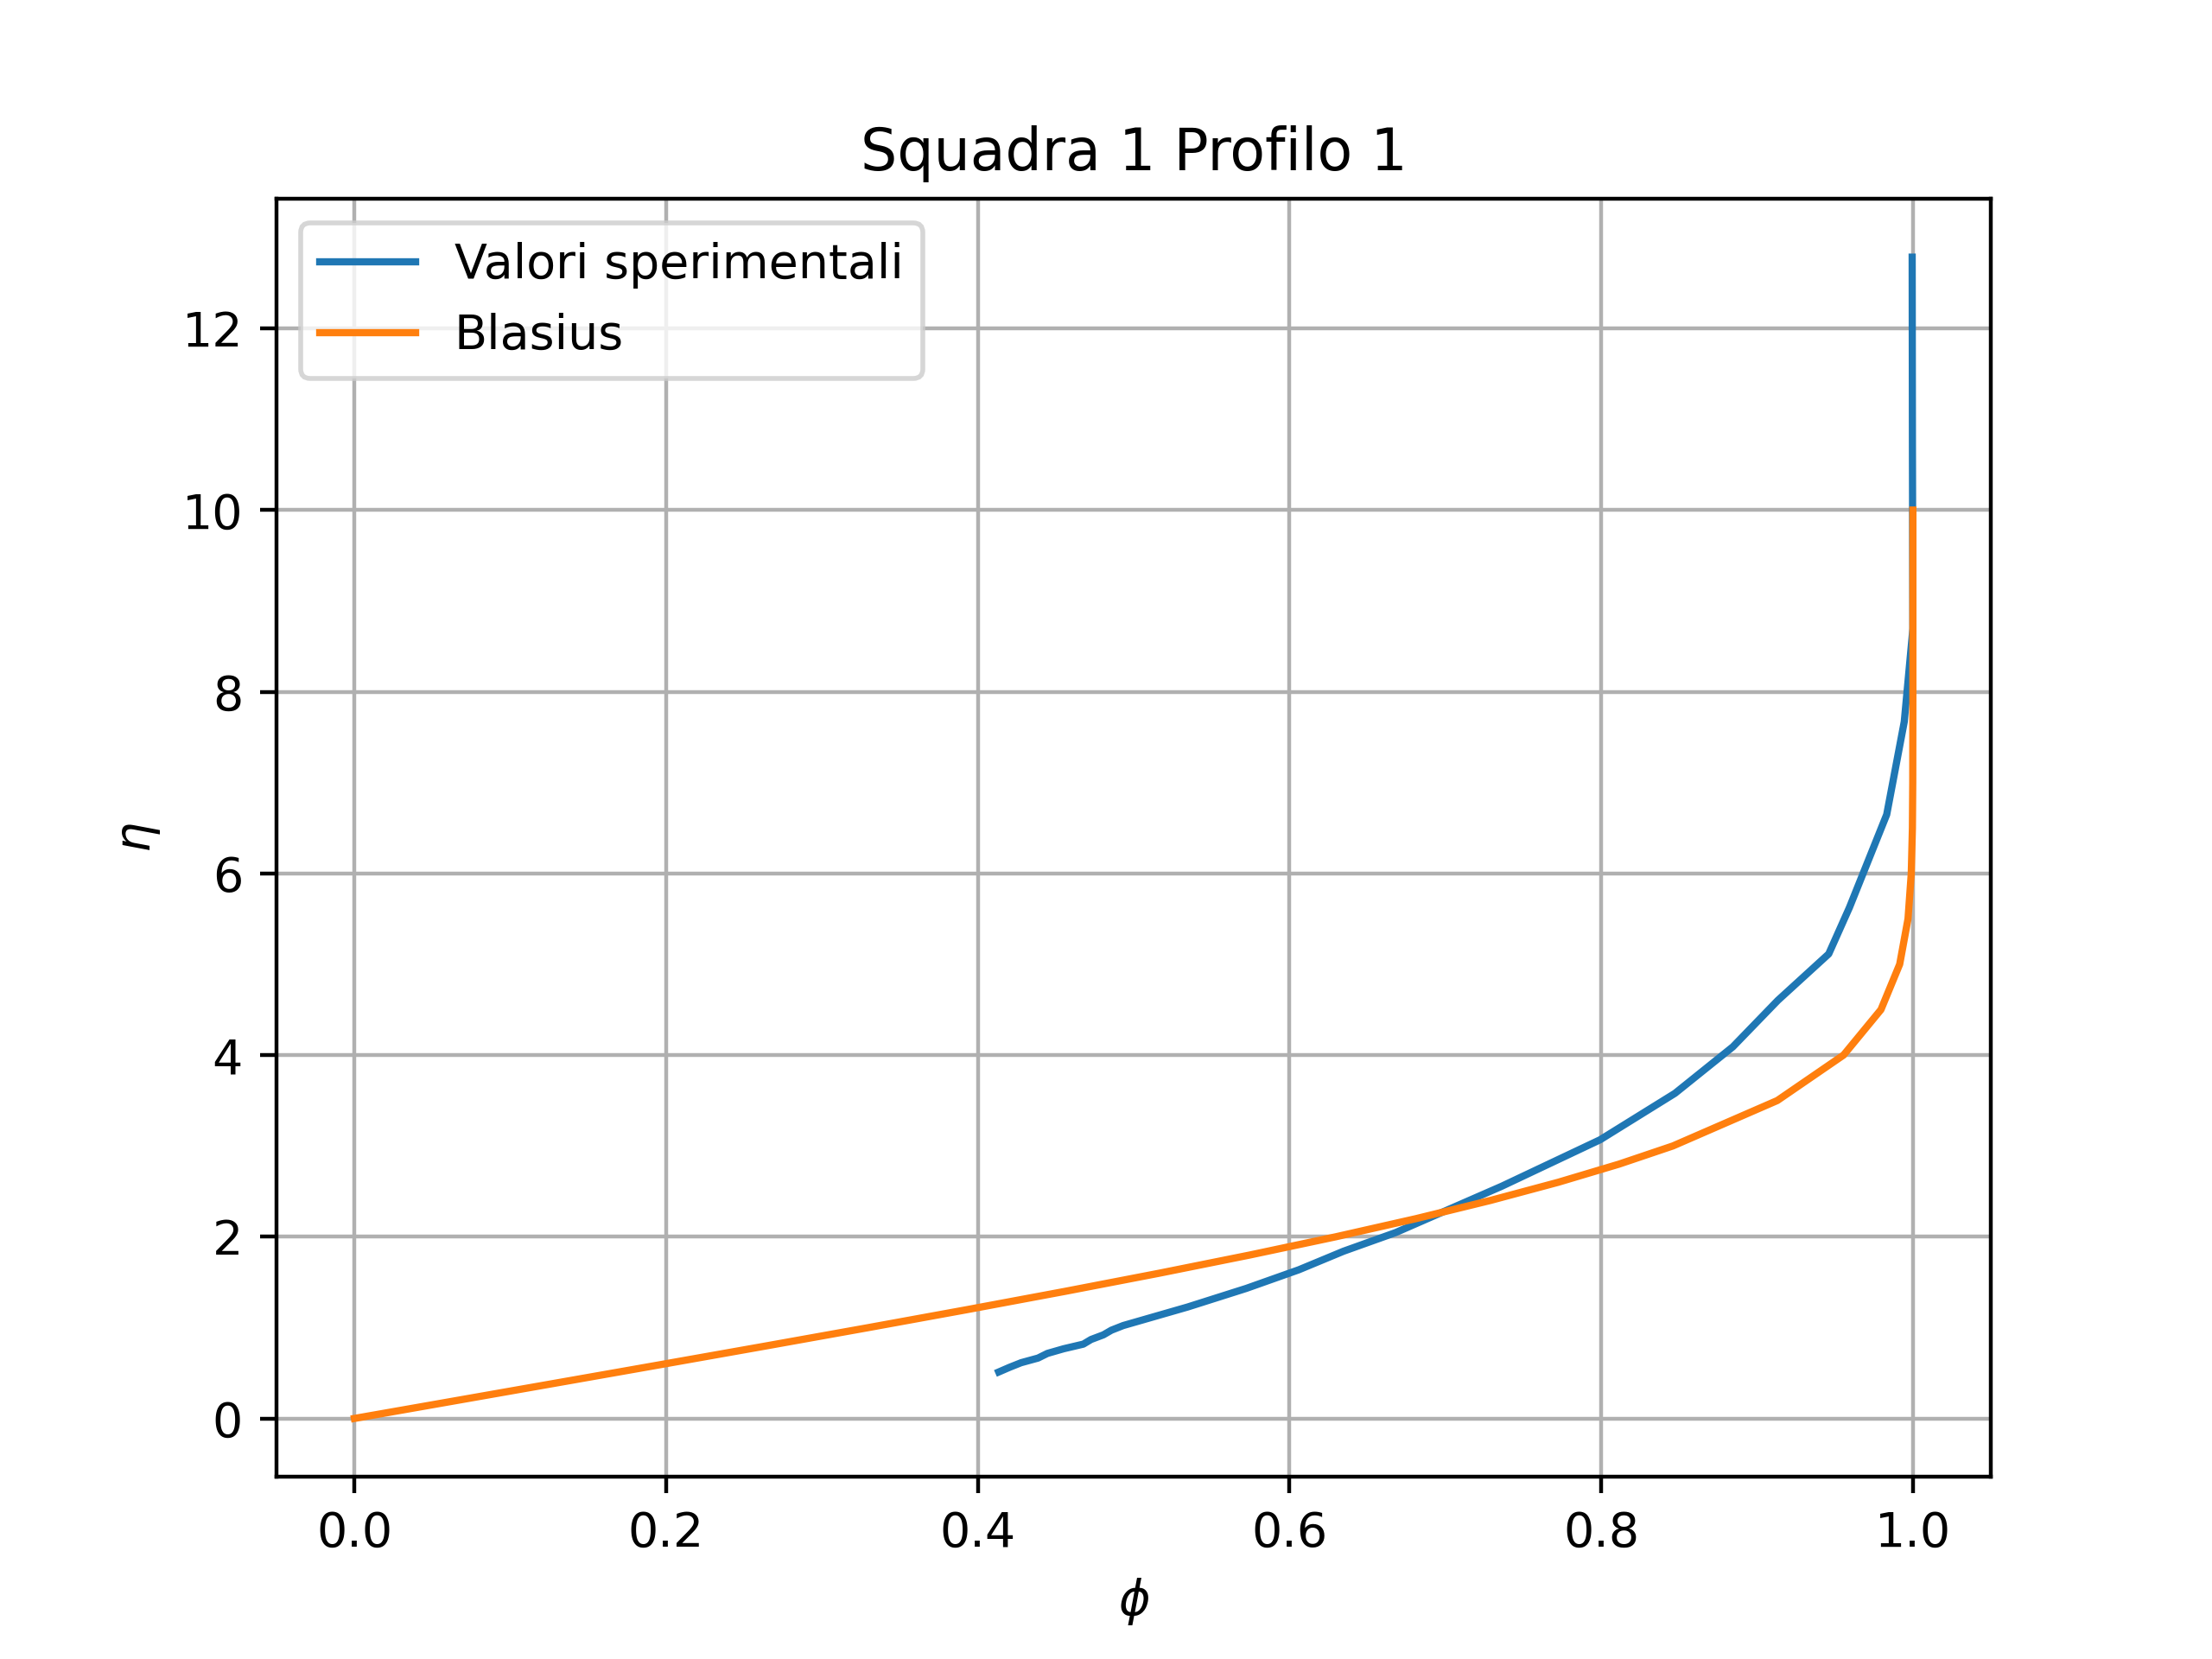
\includegraphics[width=.49\textwidth]{images/9/sq1p1_blasius.png}
    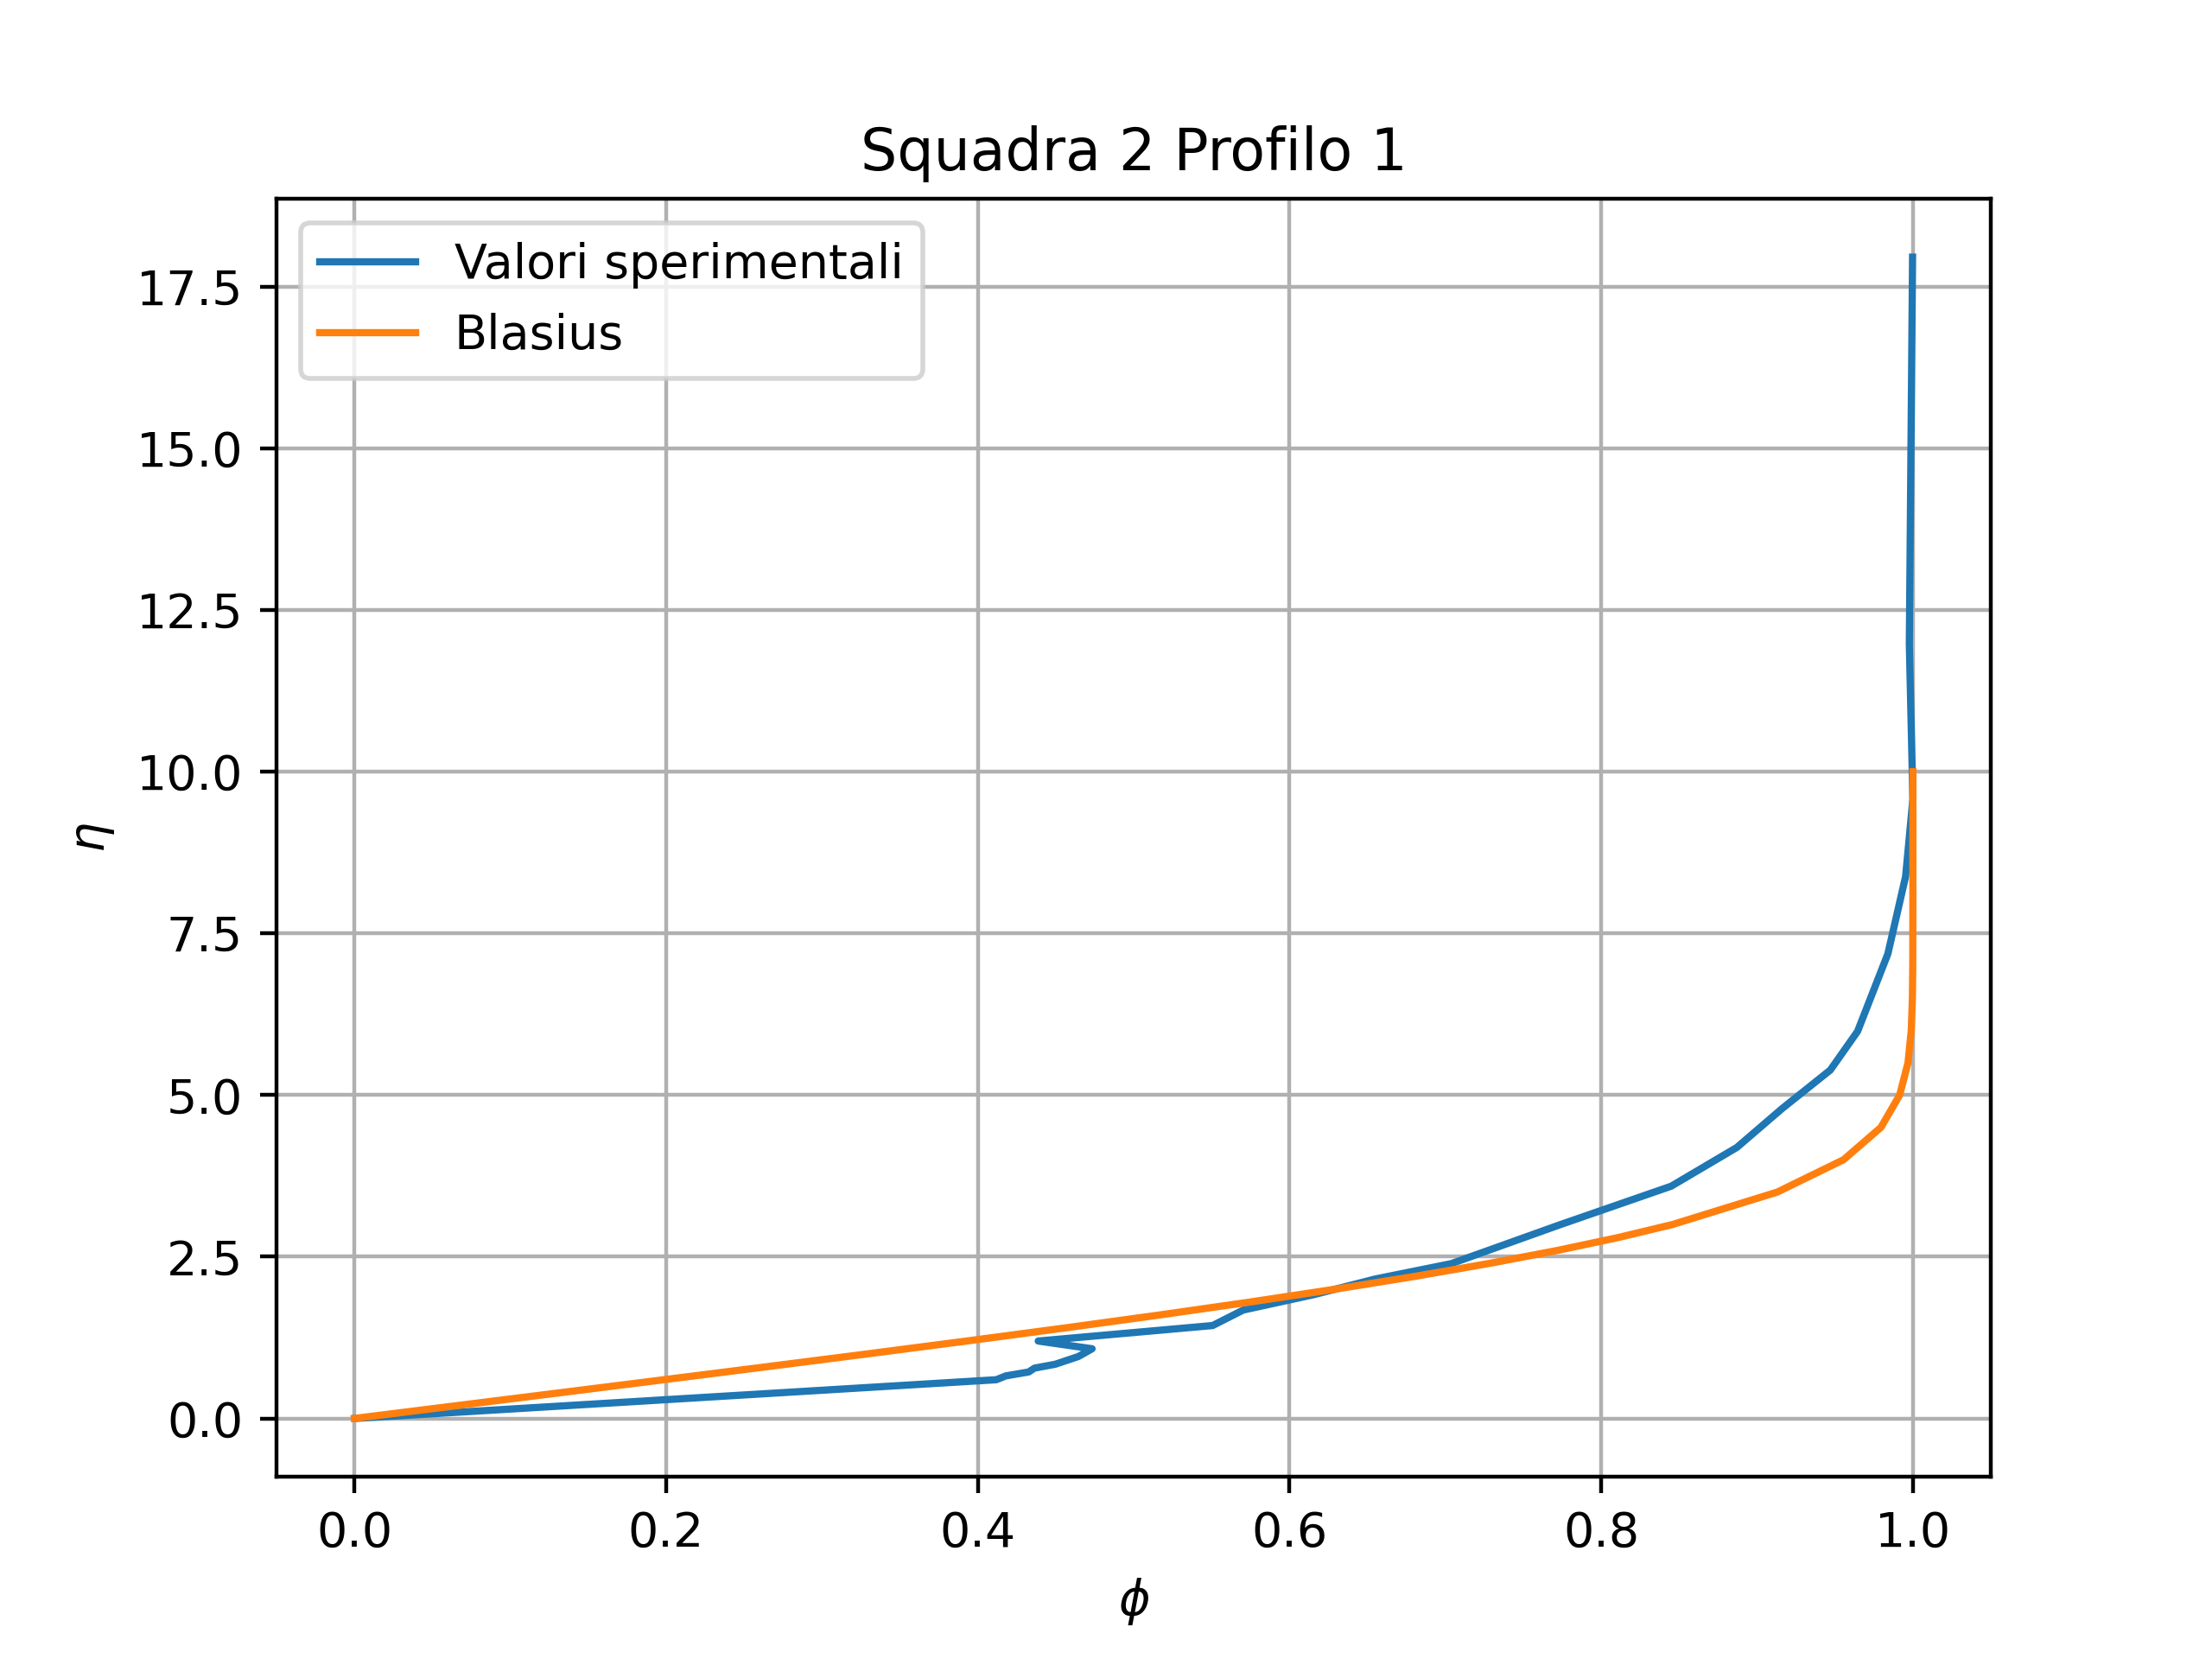
\includegraphics[width=.49\textwidth]{images/9/sq2p1_blasius.png}
    \caption{Confronto con la soluzione di Blasius, squadre 1 e 2}
\end{figure}

\begin{figure}[H]
    \centering
    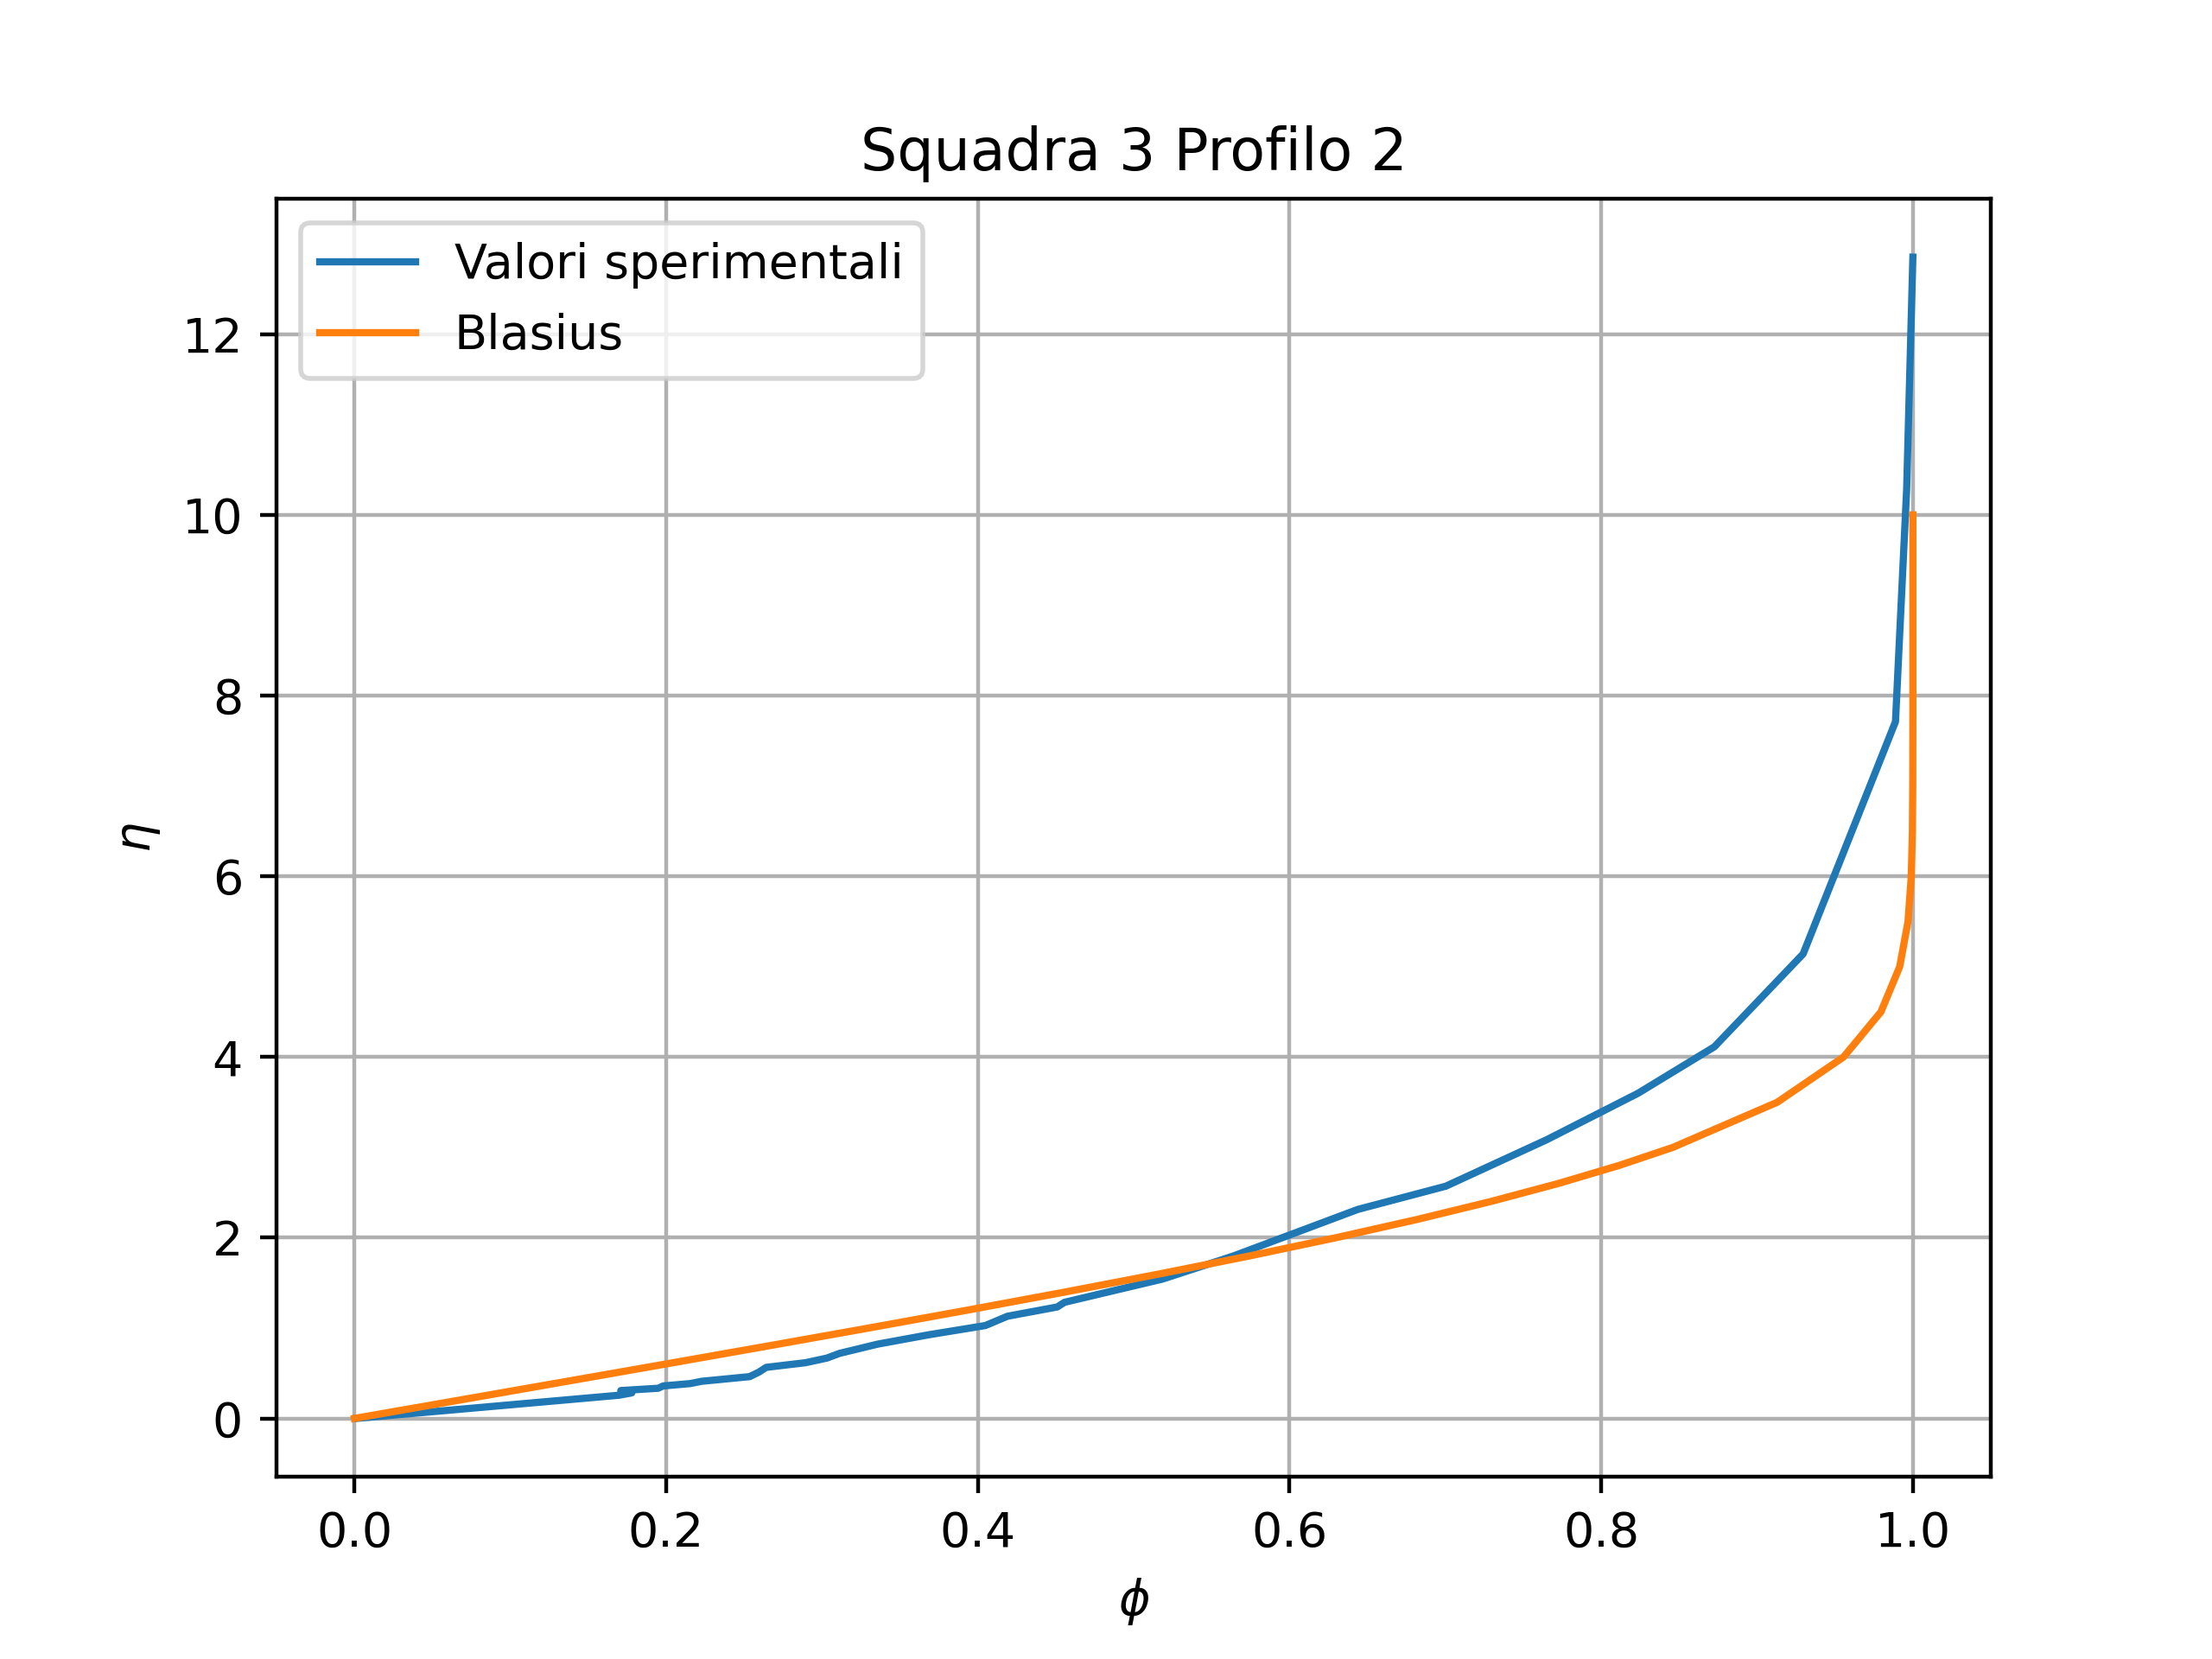
\includegraphics[width=.49\textwidth]{images/9/sq3p2_blasius.png}
    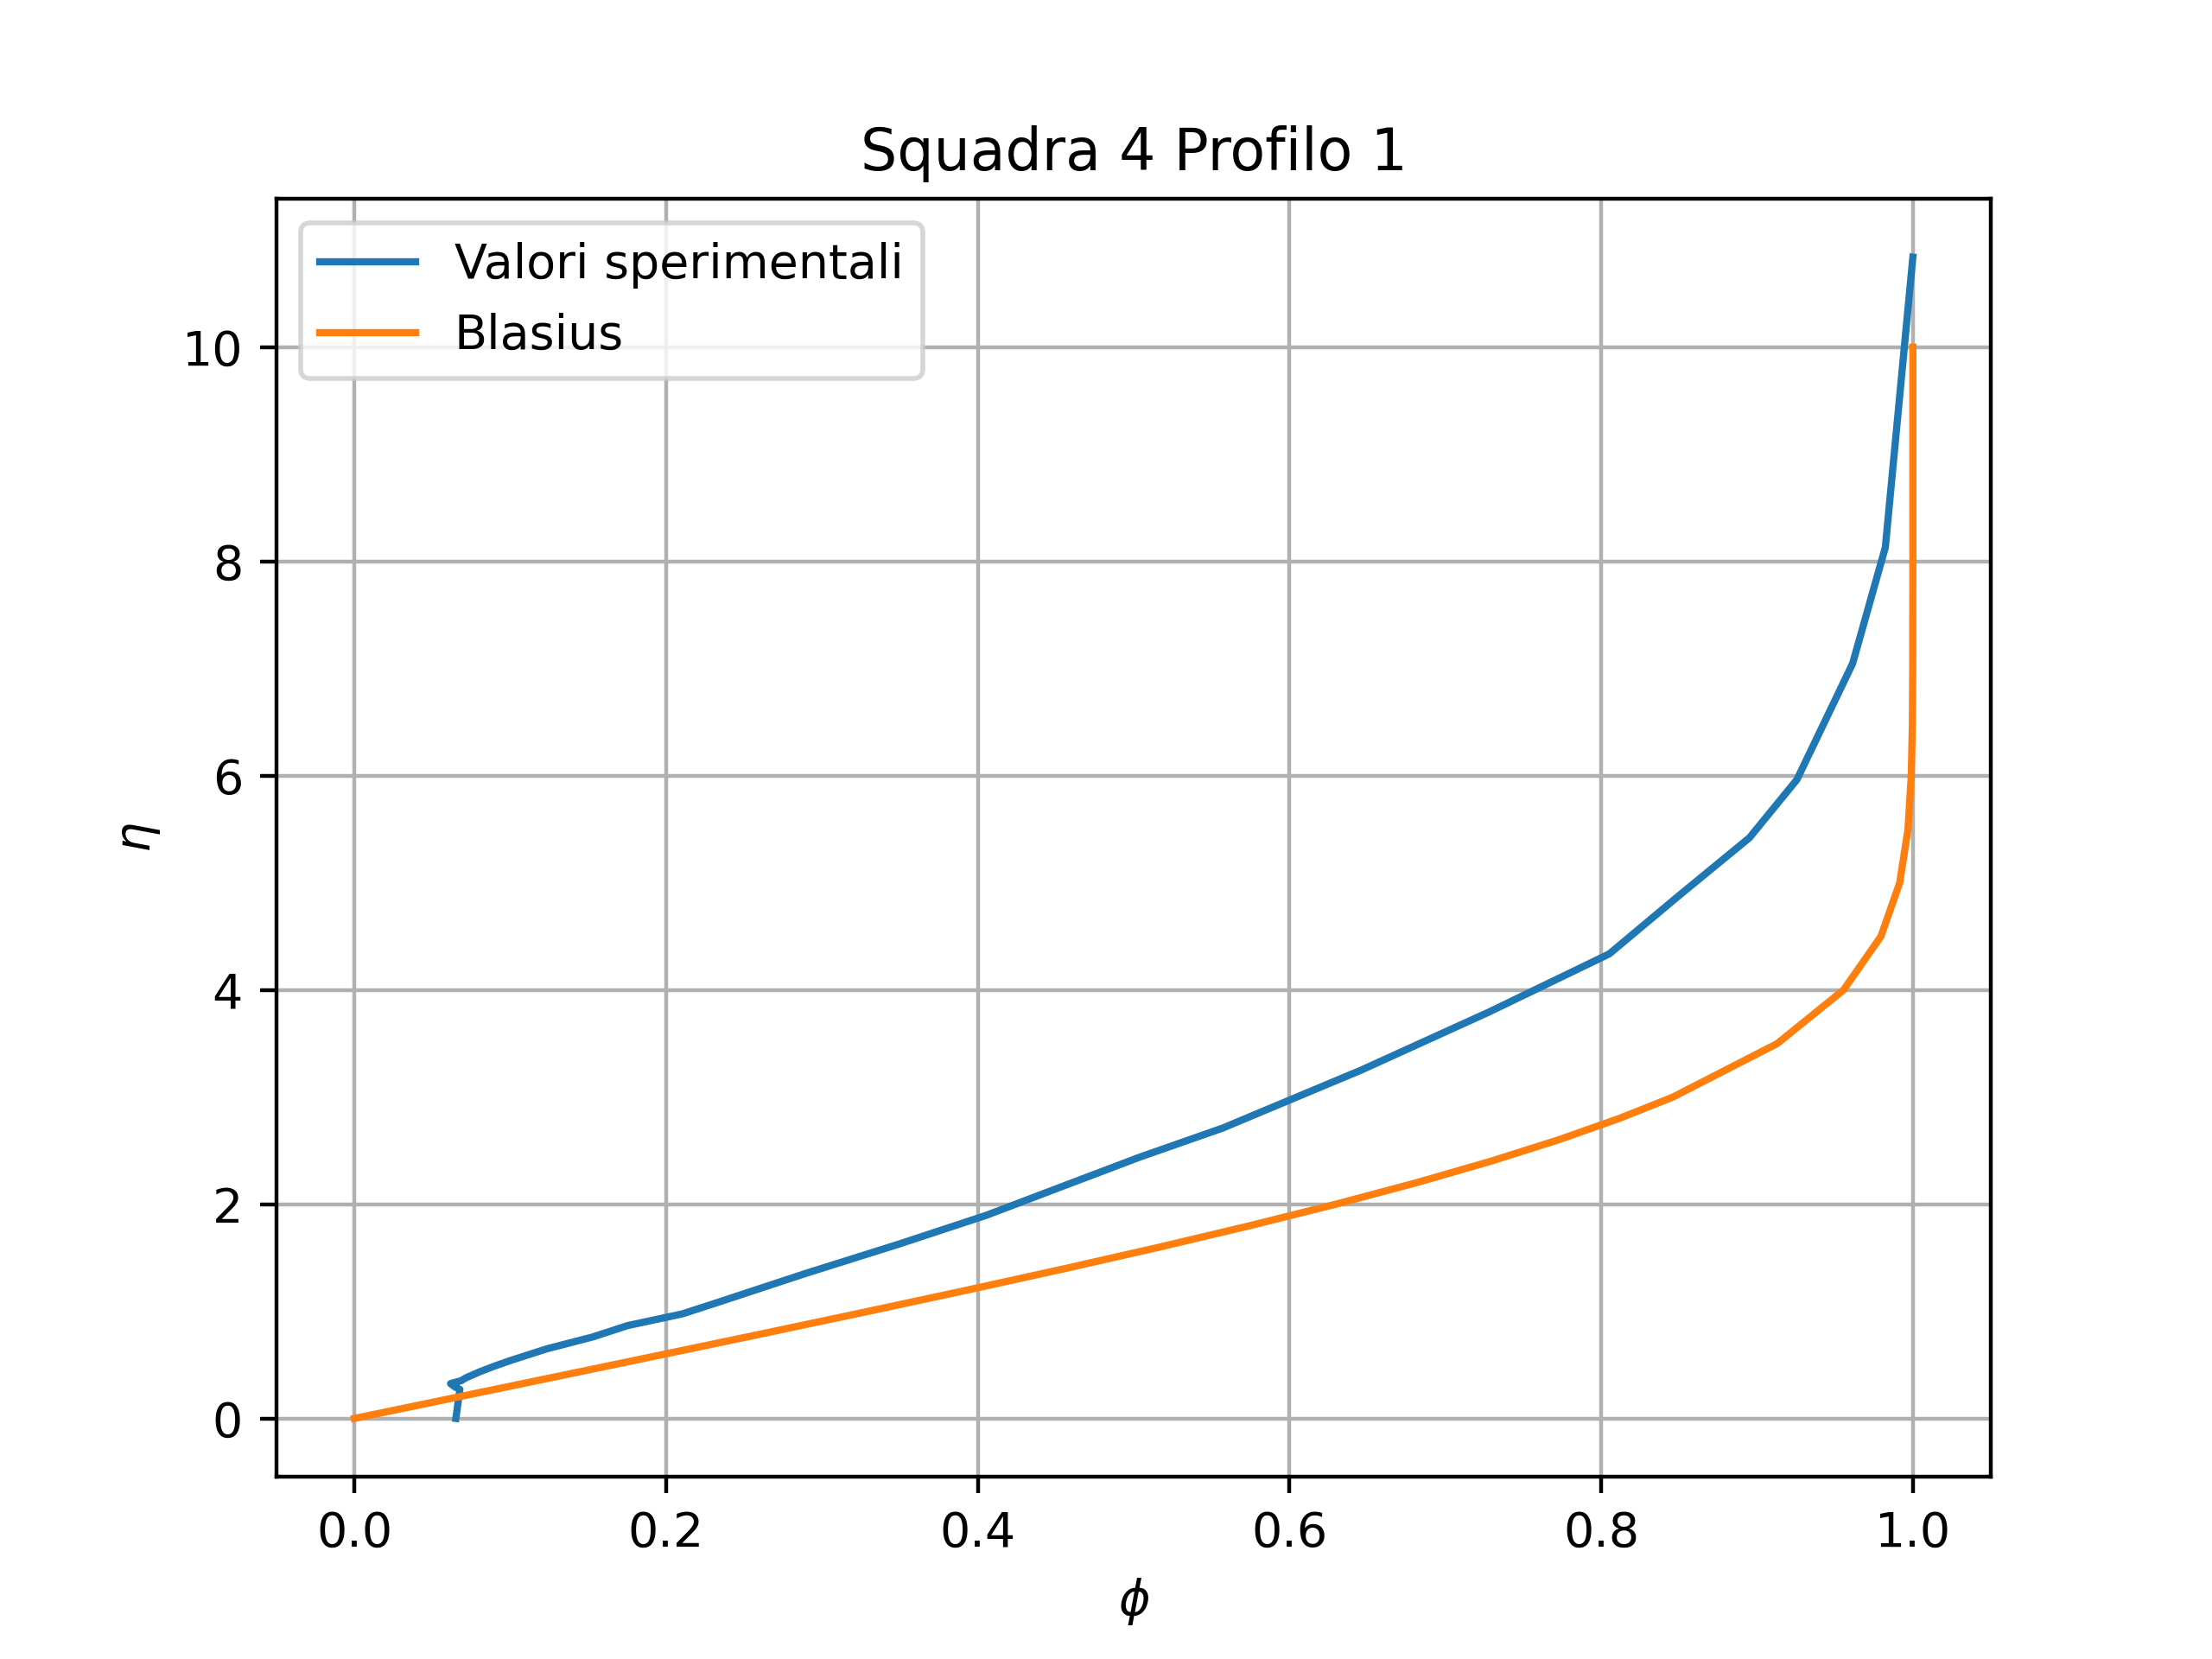
\includegraphics[width=.49\textwidth]{images/9/sq4p1_blasius.png}
    \caption{Confronto con la soluzione di Blasius, squadre 3 e 4}
\end{figure}

\noindent Si osserva come la soluzione di Blasius approssimi bene i valori dei dati sperimentali, seppur non perfettamente. La discrepanza è dovuta al fatto che nonostante il numero di Reynolds locale $Re_x$ sia inferiore al numero di Reynolds critico $Re_{cr}$, lo strato limite non sia completamente laminare bensì transizionale, e presenti quindi fenomeni di turbolenza intermittente.\\\\
L'andamento spurio che si evidenzia nei dati sperimentali per la seconda squadra è dovuto ad un'interferenza con il sostegno della sonda a filo caldo durante l'acquisizione dei dati.


% \subsection{Strato limite laminare}

% \subsubsection{Grandezze notevoli dello strato limite}
% Dal grafico di velocità media si può quindi ricavare lo spessore geometrico dello strato limite laminare $\delta = 2.2 \ mm$.\\
% Per quanto riguarda lo spessore di spostamento:

% \begin{equation*}
%     \delta^* = \int_{\infty}^{0} \left(1 - \frac{u}{U_e}\right) \, dy = 3.449
%  \ mm
% \end{equation*}

% Lo spessore di quantità di moto

% \begin{equation*}
%     \theta = \int_{\infty}^{0} \frac{u}{U_e} \cdot\left(1 - \frac{u}{U_e}\right) \, dy = 1.918 \ mm
% \end{equation*}

% E infine il parametro di forma

% \begin{equation*}
%     H = \frac{\delta^*}{\theta} = 1.798 \ mm
% \end{equation*}

% \subsubsection{Profili di velocità media e fluttuazioni adimensionali}

% Vengono presentate le velocità medie e le fluttuazioni adimensionalizzate rispettivamente come 

% \begin{equation*}
%     \frac{u}{U_{\infty}} = f \left( \frac{y}{\delta} \right)
% \end{equation*}

% \begin{equation*}
%     \frac{u_{\text{rms}}}{U_{\infty}} = f \left( \frac{y}{\delta} \right)
% \end{equation*}

% \subsubsection{Confronto con la teoria di Blausius}
% Viene costruita una variabile adimensionale $\eta = \frac{y}{\delta}$ con $\delta$ spessore geometrico.\\
% E' possibile quindi esprimere le equazioni del moto come

% \begin{equation*}
%     ff^{''} + 2 f^{'''} = 0
% \end{equation*}

% con $f = f(\eta)$ e $f^{'} = \frac{u}{U_\infty}$. Si ottiene una soluzione tabulata che viene riportata in appendice. Si denota comunque che fino a un certo numero di Reynolds, cioè fino a quando lo strato limite è da considerarsi laminare, si ha una soluzione unica per i profili di velocità. E' come se il flusso fosse self-similare.\\
% Di seguito viene presentato il confronto tra i dati sperimentali e la soluzione di Blausius

% \subsection{Strato limite turbolento}
% \subsubsection{Profilo di velocità media e fluttuazioni di velocità}
% Si presentano i profili dei sperimentali relativi alle velocità medie e alle fluttuazioni di velocità

% \subsubsection{Grandezze notevoli dello strato limite}
% Dal grafico di velocità media anche per il caso turbolento si può ricavare lo spessore geometrico dello strato limite laminare $\delta = 5.05 \ mm$.\\
% Per quanto riguarda lo spessore di spostamento:

% \begin{equation*}
%     \delta^* = \int_{\infty}^{0} \left(1 - \frac{u}{U_e}\right) \, dy = 0.204 \ mm 
% \end{equation*}

% Lo spessore di quantità di moto

% \begin{equation*}
%     \theta = \int_{\infty}^{0} \frac{u}{U_e} \cdot\left(1 - \frac{u}{U_e}\right) \, dy = 1.7 \ mm
% \end{equation*}

% E infine il parametro di forma

% \begin{equation*}
%     H = \frac{\delta^*}{\theta} = 1.201 \ mm
% \end{equation*}

% \subsubsection{Profili di velocità media e fluttuazioni adimensionali}

%  Le velocità medie e le fluttuazioni adimensionalizzate nel caso turbolento con la medesima adimensionalizzazione del caso laminare si presentano come:

% \subsubsection{Diagramma con variabili interne dello strato limite}
% Si sfrutta il Metodo di Clauser per tracciare i profili di velocità media e delle fluttuazioni adimensionalizzati con le variabili interne dello strato limite.

% \begin{equation*}
%     u^+ = \frac{\Bar{U}}{u_\tau} = f(y^+)
% \end{equation*}

% \begin{equation*}
%     \frac{u_{rms}}{u_\tau} = f(y^+)
% \end{equation*}

% Le variabili interne dello strato limite turbolento si definiscono come:

% \begin{equation*}
%     y^+ = \frac{y}{l_\tau}
% \end{equation*}

% \begin{equation*}
%         l_\tau = \frac{\nu}{u_\tau} \\
% \end{equation*}

% \begin{equation*}
%     u_\tau = \frac{\tau _w}{\rho} = U_e \sqrt{\frac{Cf}{2}}
% \end{equation*}
% Attraverso il metodo di Clauser è possibile determinare il valore del coefficiente di sforzo d'attrito a parete $C_f = \frac{\tau _w}{\frac{1}{2}\rho U^2_e}$.\\
% In questo metodo viene sfruttato il log layer per conoscere lo strato interno dello strato limite turbolento e quindi per determinare in modo sommario lo sforzo d'attrito a parete. Infatti nel log layer c'è la possibilità di avere più misurazioni che inoltre sono più accurate.\\
% Sfruttando quindi la relazione della velocità nel sottostrato logaritmico 

% \begin{equation*}
%     u^+ = \frac{1}{k}logy^+ + C
% \end{equation*}

% con k = 0.41 (costante di VonKarman) e C = 5.1 (costante di Coles). Utilizzando le relazione di $u^+$ e $y^+$ si ottiene la seguente formulazione:

% \begin{equation*}
%     \frac{u}{U_e} = \sqrt{\frac{Cf}{2}}\left[\frac{1}{k}\left(log\frac{yU_e}{\nu} + log\sqrt{\frac{C_f}{2}}\right) + C\right]
% \end{equation*}

% Viene quindi costruita la mappa di Clauser assumendo differenti valori di $C_f$. Sovrapponendo il profilo di velocità sperimentale si osserva quale $C_f$ si avvicina maggiormente ai dati sperimentali.

% Si ricava quindi il $C_f = 0.0045$ con il quale si rappresenta l'andamento della velocità e delle fluttuazioni all'interno dello strato limite

% \begin{equation*}
%     u^+ = \frac{U}{u_\tau}
% \end{equation*}

% \begin{equation*}
%     y^+ = \frac{y}{l_\tau}
% \end{equation*}

% Si ottiene quindi il seguente diagramma per la velocità adimensionale rispetto alla coordinata interna


% Per quanto riguarda le fluttuazioni invece:

% \subsection{Confronto strato limite laminare e turbolento}

% In primo luogo si evidenzia il confronto tra i valori notevoli dello strato limite laminare e turbolento:


% Vengono dati anche i grafici di confronto tra gli andamenti dello strato limite laminare e turbolento per la velocità media, le fluttuazioni turbolente e i valori adimensionali.